\documentclass[aps,pra,preprint,superscriptaddress,amsmath,amssymb]{revtex4-2}
\usepackage{graphicx}
\graphicspath{{./figures/}}
\usepackage{booktabs,braket}
\usepackage{tabularx}
% Pin array.sty: REVTeX 4.2 + tabularx breaks with array >= 2.5 (Extra \or).
% Bundled array.sty (v2.4d, 2016) shadows the TeX distribution copy.
\makeatletter
\@ifpackagelater{array}{2016/10/07}{%
  \PackageError{array}{Newer array package detected. tabularx is incompatible
    with REVTeX 4.2 for array >= 2.5. Use the bundled array.sty v2.4d shipped in
    this project directory}{}%
}{}%
\makeatother
\usepackage{siunitx}
\usepackage{xr}
\usepackage[colorlinks=true,citecolor=blue,linkcolor=blue,urlcolor=blue]{hyperref}
\usepackage[capitalize]{cleveref}
\externaldocument[MAIN-]{01_track_A_topo_main}
\sisetup{
  retain-unity-mantissa = false,
  exponent-product = \times,
}
\renewcommand{\theequation}{S\arabic{equation}}
\renewcommand{\thefigure}{S\arabic{figure}}
\renewcommand{\thetable}{S\arabic{table}}
\renewcommand{\thesection}{S\arabic{section}}
\newcommand{\dd}{\mathrm{d}}
\providecommand{\ketbra}[2]{|#1\rangle\langle#2|}

\setlength{\emergencystretch}{1.5em}
\begin{document}

\title{Supplemental Material for ``Finite-size and loss-profile limits on topological protection of Wigner negativity in a chiral Floquet SSH chain''}

\author{Juste Deuyekbe}
\affiliation{Department of Physics, Faculty of Science, University of Ngaoundere, P.O. Box 454, Ngaoundere, Cameroon}

\author{P. Djorw\'e}
\email{djorwepp@gmail.com}
\affiliation{Department of Physics, Faculty of Science, University of Ngaoundere, P.O. Box 454, Ngaoundere, Cameroon}
\affiliation{Stellenbosch Institute for Advanced Study (STIAS), Wallenberg Research Centre at Stellenbosch University, Stellenbosch 7600, South Africa}

\author{A.-H. Abdel-Aty}
\email{amabdelaty@ub.edu.sa}
\affiliation{Department of Physics, College of Sciences, University of Bisha, Bisha 61922, Saudi Arabia}

\author{A. Elrashidi}
\email{a.elrashidi@ubt.edu.sa}
\affiliation{College of Engineering, University of Business and Technology, Jeddah 21448, Saudi Arabia}

\author{Nsangou Mama}
\email{mnsangou@yahoo.com}
\affiliation{Department of Physics, Faculty of Science, University of Maroua, P.O.Box 46, Maroua, Cameroon}

\author{S. G. Nana Engo}
\email{serge.nana-engo@facsciences-uy1.cm}
\affiliation{Department of Physics, Faculty of Science, University of Yaounde I, P.O.Box 812, Yaounde, Cameroon}

\maketitle

% ======================================================================
\section{Scope and numerical design}
\label{sec:scope}

This Supplemental Material specifies the model, protocol, and uncertainty analyses behind the main-text boundary statement, treating the laboratory-frame Wigner observable separately from the micromotion-covariant edge-mode observable. The conclusions apply to the stated finite-time Kerr--Lindblad model and do not establish a protection theorem, a hardware operating point, or a metrological gain.

% ======================================================================
\section{Two-step chiral model}
\label{sec:model}

For a unit cell containing sublattices $A$ and $B$, the bulk Hamiltonian is
\begin{equation}\label{eq:bulk}
H(k)=\left(J_A+J_B\cos k\right)\sigma_x+J_B\sin k\,\sigma_y,
\end{equation}
with chiral operator $\Gamma=\sigma_z$. The drive consists of
\begin{equation}\label{eq:drive}
H(t)=\begin{cases}
H_A,&0\leq t<T/2,\\
H_B,&T/2\leq t<T,
\end{cases}
\qquad T=2\pi,
\end{equation}
where $H_A$ contains only the intracell hopping and $H_B$ only the intercell hopping. The period propagator is
\begin{equation}\label{eq:uf}
U_F(k)=\exp[-iH_B(k)T/2]\exp[-iH_A(k)T/2].
\end{equation}

The two symmetric time frames produce off-diagonal winding numbers $w_A$ and $w_B$~\cite{Asboth2014}. We report
\begin{equation}\label{eq:nu}
\nu_0=(w_A+w_B)/2,\qquad \nu_\pi=(w_A-w_B)/2.
\end{equation}
The selected chiral point $(J_A,J_B)=(\num{0.1},\num{1.2})$ has $(\nu_0,\nu_\pi)=(-1,0)$; the selected trivial point $(\num{1.2},\num{0.1})$ has $(0,0)$. The maximum chiral-frame residual is below $\num{1e-15}$ on the resolution ladder. The minimum zero and $\pi$ gaps are positive at both points. The phase structure and finite-chain edge diagnostic are summarized in \cref{fig:phase}.

\begin{figure}[t]
  \centering
  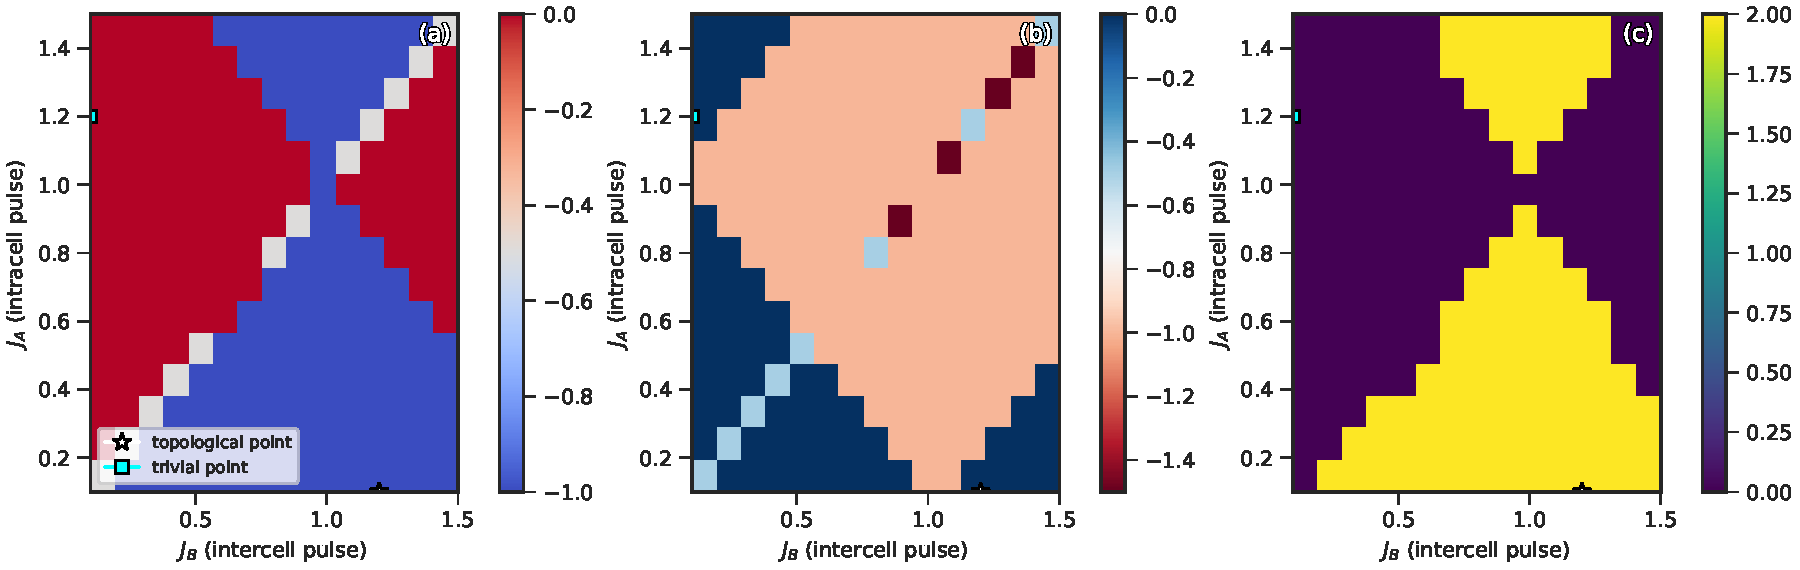
\includegraphics[width=0.98\linewidth]{chiral_floquet_phase_audit.pdf}
  \caption{Coherent phase structure. (a)~Integer Floquet invariant $\nu_0$. (b)~Minimum quasienergy gap with working points marked (filled: chiral; open: trivial). (c)~Finite-chain edge diagnostic. Working points are chosen from the invariant and gap criteria before any dissipative simulation.}
  \label{fig:phase}
\end{figure}

For an open chain, the single-particle propagator is constructed from the same step Hamiltonians. The edge vector $u_e(0)$ used in the edge-mode analysis is the most edge-localized eigenvector of the one-period open-chain propagator for the chiral point. This observable is distinct from the bulk invariant and is not assigned an open-system topological index.

{\sloppy The working points tested in an earlier draft, specifically $(J_A,J_B)=(\num{1.0},\num{1.0})$ and the $N=\num{6}$ point, were not retained because the trivial-sector winding and the finite-chain invariant were not resolution-stable under independent recomputation. The current working points were selected de novo from the phase scan using the invariant and gap criteria described above.\par}

% ======================================================================
\section{Dissipative dynamics}
\label{sec:dynamics}

The bosonic open-chain evolution is
\begin{equation}\label{eq:lindblad}
\dot\rho=-i[H(t)+H_{\rm K},\rho]
+\sum_j\gamma_j\left(a_j\rho a_j^\dagger-\frac{1}{2}a_j^\dagger a_j\rho-\frac{1}{2}\rho a_j^\dagger a_j\right),
\end{equation}
with the local Kerr term $H_{\rm K}=\chi\,a_1^{\dagger 2}a_1^2$, $\chi=\num{0.5}$. The primary starts from a normalized even cat state $\ket{\alpha}+\ket{-\alpha}$ with $\alpha=\num{1.0}$ on the boundary site. The mode-resolved preparation distributes the displacement along the single-particle edge vector, $\alpha_j=\alpha\,u_{e,j}(0)$; both preparations are used identically for the two sectors. The local Fock cutoff is $N_{\max}=\num{2}$. The edge-low-loss profile uses $\gamma_{\rm edge}=\num{1e-4}$ at the two boundary sites and $\gamma_{\rm bulk}=\num{0.2}$ elsewhere; the uniform profile uses the bulk rate at all sites. Multiplicative rate perturbations use one factor $\xi\sim\mathcal{U}(-d,d)$ per realization, applied to every site ($\gamma_j\to\gamma_j(1+\xi)$), at four declared levels; perturbed rates are clamped at zero.

The Lindblad equation is integrated with the quantum-jump (Monte Carlo wave-function) trajectory method~\cite{Dalibard1992} via QuTiP~\cite{Johansson2013} (5.3.1, numpy 1.26.4), with integrator step budget $\num[retain-unity-mantissa = false]{1e4}$, final-state storage, nine output times over one period. The primary analysis uses ten trajectories per realization and the edge-mode analysis five; trajectories are nested within each realization and the realization is the independent unit.

The integrated negative volume of the reduced local Wigner function is
\begin{equation}\label{eq:neg}
\delta_{-}(t)=\int\!\int\frac{|W(q,p;t)|-W(q,p;t)}{2}\,\dd q\,\dd p,
\end{equation}
on a $\num{31}\times\num{31}$ grid over $[-4,4]^2$, evaluated after one period. Wigner negativity admits operational witnesses beyond a finite phase-space integral~\cite{Chabaud2021witnessingwigner,Zaw2024}.

\begin{table}[h]
\caption{Fixed simulation parameters. All dynamical parameters are normalized model coordinates, not an SI calibration.}
\label{tab:parameters}
\begin{ruledtabular}
\begin{tabular}{lll}
Quantity & Main dynamics & Covariant analysis \\
\hline
Cells/modes & \num{2}/\num{4}, \num{3}/\num{6}, \num{4}/\num{8} & \num{2}/\num{4} \\
$N_{\max}$ & \num{2} & \num{2} \\
$\chi$ & \num{0.5} & \num{0} or \num{0.5} \\
$n_{\rm MC}$ & \num{500}, \num{500}, \num{2000} & \num{10} \\
Trajectories/unit & \num{10} & \num{5} \\
Wigner grid & $\num{31}\times\num{31}$ & $\num{31}\times\num{31}$ \\
Solver & QuTiP mcsolve 5.3.1 & QuTiP mcsolve 5.3.1 \\
Integrator steps & \num[retain-unity-mantissa = false]{1e4} & \num[retain-unity-mantissa = false]{1e4} \\
Stored output times & \num{9} & \num{17} \\
Observation window & $T=2\pi$ & $\num{8}T$ \\
Independent unit & disorder draw & matched disorder draw \\
\end{tabular}
\end{ruledtabular}
\end{table}

% ======================================================================
\section{Matched analysis, uncertainty, and paired comparison}
\label{sec:statistics}

For each profile, disorder level, and realization $r$, the sector contrast is
\begin{equation}\label{eq:contrast}
\Delta_r=Y_{r,{\rm chiral}}-Y_{r,{\rm trivial}},
\end{equation}
formed inside each matched disorder draw before aggregation. The summary is the mean of $\Delta_r$ and a bootstrap percentile \qty{95}{\percent} interval~\cite{Efron1979} over the independent realization units ($\num[retain-unity-mantissa = false]{1e4}$ resamples, seeded). Sector simulations share the disorder draw, initial state, cutoff, grid, and loss rates; their trajectory seeds are distinct but derived deterministically from the draw seed. This paired construction avoids treating repeated trajectory values or time points as independent replicates. No p-value is used as evidence of protection, and contrasts are not subjected to a significance test, with three narrow exceptions: (i) solver-level sign resolutions are confirmatory tests with pre-committed designs (the four-cell trajectory expansion used $\num{200}$ draws, confirmed on the trigger-independent subset, samples $\num{25}$--$\num{199}$, $-\num{0.000333}\pm\num{0.000122}$); (ii) all other intervals, trajectory ladders, longtime series, witness and cutoff strata, are exploratory and unadjusted, and no protection claim rests on any single one; (iii) all runs share one seed base ($\num{20260814}$), the paired construction cancels seed effects in the contrasts, and no multi-seed rerun was performed.

The primary comparison comprises \num{4000} matched units at two and three cells and \num{16000} at four cells, i.e.\ $N_{\rm MC}=\num{500}$, \num{500}, and \num{2000} per disorder level and loss profile; earlier four-cell runs with smaller $N_{\rm MC}$ are retained for nested comparison. The covariant analysis uses \num{80} paired units per condition.

\begin{table}[h]
\caption{Primary counts and edge-low-loss contrast ranges across the four disorder levels. Ranges are not confidence intervals.}
\label{tab:paired-comparison}
\begin{ruledtabular}
\begin{tabular}{lrrr}
Cells & Modes & $n_{\rm units}$ & Mean contrast range \\
\hline
\num{2} & \num{4} & \num{4000} & $\num{+0.0131}$ to $\num{+0.0167}$ \\
\num{3} & \num{6} & \num{4000} & $\num{-0.0023}$ to $\num{-0.0020}$ \\
\num{4} & \num{8} & \num{16000} & $\num{-0.0021}$ to $\num{-0.0018}$ \\
\end{tabular}
\end{ruledtabular}
\end{table}

Under uniform loss the mean contrasts are near zero or weakly negative. Because the sign changes with size, the local observable is not treated as a protection signature (prespecified criterion).

% ======================================================================
\section{Micromotion-covariant edge-mode observable}
\label{sec:covariantmethod}

The analysis defines
\begin{equation}\label{eq:covariant}
u_e(t)=U_{\rm coh}(t)u_e(0),\qquad
b_e(t)=\sum_j u_{e,j}(t)^*a_j,
\qquad n_e(t)=\braket{b_e^\dagger(t)b_e(t)}.
\end{equation}
The number-operator coefficients are $u_{e,i}(t)u_{e,j}(t)^*$ in the $a_i^\dagger a_j$ basis. A fixed-frame number operator is retained as a negative control; the covariant operator is used for the edge-mode interpretation.

The time-dependent passive exposure is
\begin{equation}\label{eq:exposure}
\Gamma_e(t)=\int_0^t\gamma_e(s)\dd s,
\qquad \gamma_e(s)=\sum_j\gamma_j|u_{e,j}(s)|^2,
\end{equation}
with reference $n_e(0)\exp[-\Gamma_e(t)]$. This equality is exact only in an isolated passive mode with no edge--bulk transfer. We prespecified a decision threshold of $\num{1e-3}$ on the maximum absolute residual of the conditional passive reference. The covariant analysis yielded maximum residuals of \num{0.03956} (common-site) and \num{0.38257} (mode-resolved); both violate the threshold by roughly $\num{40}\times$ and $\num{380}\times$, computed over \num{10} independent disorder realizations per condition. The median residual across the \num{10} realizations is \num{0.021} (common-site) and \num{0.27} (mode-resolved), still above the \num{1e-3} threshold. The residual panel is non-monotone in the Fock cutoff: maximum residuals of \num{0.0388}, \num{0.0282}, \num{0.0356} at $N_{\max}=\num{2},\num{3},\num{4}$ (Kerr-free reference), so cutoff convergence of the passive reference is not established. Results are shown in \cref{MAIN-fig:covariant}.

\subsection{Mechanistic observables and their interpretation}
\label{sec:mechanisticobservables}

For a normalized single-particle edge vector $u_e(t)$, the edge weight and the site-resolved dissipative current are
\begin{equation}\label{eq:mechanismobs}
L_e(t)=\sum_{j\in\mathcal{E}}|u_{e,j}(t)|^2,
\qquad I_j(t)=\gamma_j\langle a_j^\dagger a_j\rangle_t,
\end{equation}
where $\mathcal{E}$ denotes boundary sites. These quantities test whether an edge-localized mode is less exposed to the specified loss profile; they do not establish mediation or causality, which would require a matched perturbation. In the present study the passive-reference and decoupling controls do not pass, so the recorded currents are diagnostic rather than evidence for a mechanism.

% ======================================================================
\section{Deterministic benchmarks}
\label{sec:unitarybenchmark}

Two exactly solvable controls validate the observable implementation. (i)~A single-particle unitary benchmark with losses, Kerr terms and disorder set to zero: for $N=\num{4},\num{6},\num{8},\num{12}$, the transported edge vector $u_e(t)=U_{\rm coh}(t)u_e(0)$ and an orthogonal complement basis give a maximum covariant-population error of $\num{1.33e-15}$ and a maximum edge--bulk overlap of $\num{1.42e-31}$ over \num{257} times per period. The fixed-frame population, evaluated with $u_e(0)$ instead of $u_e(t)$, falls to \num{0.895}, confirming that the micromotion correction changes the observable. (ii)~A passive single-particle decomposition with the non-Hermitian propagator
\begin{equation}\label{eq:passivepropagator}
K(t)=\mathcal{T}\exp\left[-i\int_0^t
\left(H(s)-\frac{i}{2}\sum_j\gamma_j\ketbra{j}{j}\right)\dd s\right]
\end{equation}
yields, over \num{257} times per period, a maximum reference residual of $\num{1.94e-15}$ under uniform loss (complementary-space population $\num{4.33e-16}$) and maximum residuals of \num{9.79e-4}, \num{1.94e-4}, \num{1.94e-4}, \num{1.94e-4} for \num{2}, \num{3}, \num{4}, \num{6} cells under edge-selective loss. The deterministic control shows that structured loss and micromotion are not separable in the finite chain, whereas uniform loss is. Neither benchmark establishes a resource-protection mechanism.

% ======================================================================
\section{Numerical convergence of the local observable}
\label{sec:convergence}

All checks use the two-cell system at zero disorder, $\chi=\num{0.5}$, and the primary parameters of \cref{tab:parameters}. They constrain numerical uncertainty without claiming a converged prediction.

\subsection{Wigner-grid convergence}

For a fixed final state (one realization, \num{200} trajectories), the single-site negativity integral over $[-4,4]^2$ takes the values \num{0.02695}, \num{0.02565}, \num{0.02680}, \num{0.02610}, \num{0.02621} on $\num{21}^2$, $\num{31}^2$, $\num{41}^2$, $\num{51}^2$, $\num{61}^2$ grids. All values lie within $\pm\qty{3}{\percent}$ of the finest estimate; the primary $\num{31}^2$ grid is within \qty{2.2}{\percent}. Grid discretization contributes a few-percent relative uncertainty to the absolute integral; matched contrasts cancel most of the residual.

\subsection{Trajectory-count sensitivity of the contrast}
\label{sec:trajcount}

Because the Wigner-negativity functional is nonlinear in the state, evaluating it on a trajectory-averaged state built from $N_{\rm traj}$ samples carries a positive bias that decays as $1/N_{\rm traj}$ and is concentrated in the near-zero sectors. At $N_{\rm traj}=\num{10}$ the exact master equation gives sector negativities \num{0.022854} (topological) and \num{0.000526} (trivial) at two cells, against Monte Carlo values \num{0.023685} and \num{0.006954}; the trivial-sector bias is the larger contribution. At three cells the exact values are \num{0.000389}/\num{0.000508} against Monte Carlo \num{0.004779}/\num{0.006883}, with the same downward direction on the contrast.

A trajectory ladder on the primary conditions (same seeds, edge-selective profile, $d=\num{0}$) is summarized in \cref{tab:trajladder}. The infinite-trajectory extrapolation validated against the exact column at two and three cells (deviations \num{6e-5} and \num{3e-5}, below the prespecified \num{5e-4} tolerance) gives $-\num{0.00034}$ and $-\num{0.00039}$ at four and five cells; the alternative weighted $C+c/N_{\rm traj}$ fit gives $-\num{0.00022}$ and $-\num{0.00018}$, so the extrapolation carries a model spread of about one-and-a-half at four cells. The direct four-cell \num{200}-trajectory point (\num{200} matched units) reads $-\num{0.00032}\pm\num{0.00011}$ with a \qty{95}{\percent} interval excluding zero; the five-cell \num{200}-trajectory point (\num{100} matched units) reads $-\num{0.00029}\pm\num{0.00015}$ with a \qty{95}{\percent} interval crossing zero. The four-cell resolution does not depend on the pilot draws that motivated the expansion, as a pre-specified confirmatory analysis on an independent subset of matched units confirms (\cref{sec:statistics}).

The same ladder at two and four periods resolves the small $2T$ reversal as a finite-trajectory artefact (exact contrast zero, MC estimate identically zero at $N_{\rm traj}=\num{50},\num{200}$) and brackets the $4T$ revival against the exact value ($+\num{0.0751}\pm\num{0.0009}$ at \num{200} trajectories against exact $+\num{0.07542}$).

\begin{table}[h]
\caption{Paired contrast versus trajectory count per disorder unit at $d=\num{0}$, edge-selective loss. The extrapolated column fits $\bar{C}=C+c/N_{\rm traj}+d/N_{\rm traj}^{2}$, validated against the exact column to within \num{6e-5} at both exactly solvable sizes. The alternative weighted fit gives $-\num{0.00022}$ and $-\num{0.00018}$ at four and five cells. The four- and five-cell $N_{\rm traj}=\num{200}$ points use \num{200} and \num{100} matched units.}
\label{tab:trajladder}
\begin{ruledtabular}
\begin{tabular}{lrrrrr}
Cells & $N_{\rm traj}=\num{10}$ & \num{50} & \num{200} & Exact ME & Extrapolated $C$ \\
\hline
\num{2}  & $+\num{0.01673}$ & $+\num{0.02042}$ & $+\num{0.02177}$ & $+\num{0.02233}$ & $+\num{0.02227}$ \\
\num{3}  & $-\num{0.00210}$ & $-\num{0.00050}$ & $-\num{0.00019}$ & $-\num{0.00012}$ & $-\num{0.00009}$ \\
\num{4}  & $-\num{0.00201}$ & $-\num{0.00032}$ & $-\num{0.00032}$ & n/a & $-\num{0.00034}$ \\
\num{5}  & $-\num{0.00218}$ & $-\num{0.00010}$ & $-\num{0.00029}$ & n/a & $-\num{0.00039}$ \\
\end{tabular}
\end{ruledtabular}
\end{table}

\subsection{Cross-solver consistency}
\label{sec:crosssolver}

The full Lindblad master equation (QuTiP \texttt{mesolve}, exact in the chosen cutoff) was integrated alongside the Monte Carlo wave-function solver (\texttt{mcsolve}) for two- and three-cell systems at zero and intermediate disorder, both sectors and both loss profiles ($N_{\max}=\num{2}$; \num{200} trajectories per MC condition at two cells, \num{800} at three). Final-time averaged states agree at two cells with mean Uhlmann fidelity $\bar{F}=\num{0.99957}$ (max trace distance \num{1.93e-2}) and at three cells with $\bar{F}=\num{0.99978}$ (max trace distance \num{2.12e-2}), with no systematic sector or profile bias. Because the negativity is a nonlinear functional of the trajectory-averaged state, the contrast is recomputed directly with both solvers: with \num{10} trajectories the Monte Carlo solver reproduces the primary records exactly (max absolute difference $\num{0}$), while the exact master equation gives $+\num{0.02233}$ against $+\num{0.01673}$ at two cells and $-\num{0.00012}$ against $-\num{0.00210}$ at three cells. The difference is the positive finite-trajectory bias quantified above.

Two additional checks bound the numerical implementation. (i)~A hierarchical-equations-of-motion (HEOM) propagation of the same Lindblad generator at three cells ($N_{\max}=\num{2}$, HEOM depth \num{1}, $T_{\rm bath}=\num{0.1}$, $\gamma_{\rm bulk}=\num{1.0}$) agrees with the exact master equation to a relative edge-population error below \qty{0.6}{\percent} in all eight sector/profile/disorder conditions (mean \qty{0.28}{\percent}). (ii)~HEOM depth convergence on the primary two-cell chain with a Drude--Lorentz bath on every site ($\lambda=\num{0.3}$, cutoff \num{1.0}, $T_{\rm bath}=\num{0.5}$, \num{2} Matsubara terms) gives one-period edge negativities \num{0.0379},\num{0.0000},\num{0.0000} (topological) and \num{0.0390},\num{0.0119},\num{0.0000} (control) at depths \num{1},\num{2},\num{3}; every depth increment shrinks, and raising the Matsubara cutoff from \num{2} to \num{3} at depth \num{1} moves the negativity by at most \num{9.1e-3}. The HEOM check is a solver-machinery cross-validation on $N=\num{3}$, not a re-validation of the primary runs.

\subsection{Kerr-free primary stratum}
\label{sec:kerrfree}

The Kerr term enters both as the resource generator and as a possible confounder: removing it separates filtering of the prepared negativity from interaction-generated effects. The full matched design was re-run at $\chi=\num{0}$ (identical seeds and disorder draws, \num{500} units per stratum, \num{10} trajectories, one period). Under edge-selective loss at $d=\num{0}$:

\begin{table}[h]
\caption{Zero-disorder edge-selective contrast at $\chi=\num{0}$ (Kerr-free) versus primary $\chi=\num{0.5}$. Master-equation values are exact; Monte Carlo values are means $\pm$ \qty{95}{\percent} half-widths over \num{500} matched draws.}
\label{tab:kerrfree}
\begin{ruledtabular}
\begin{tabular}{lrrrr}
Cells & $\chi=0$ ME & $\chi=0$ MC & $\chi=\num{0.5}$ ME & $\chi=\num{0.5}$ MC \\
\hline
\num{2} & $+\num{0.010467}$ & $+\num{0.008875}\pm\num{0.000701}$ & $+\num{0.022328}$ & $+\num{0.0167}\pm\num{0.0011}$ \\
\num{3} & $\num{0.000000}$ & $-\num{0.001254}\pm\num{0.000622}$ & $-\num{0.000119}$ & $-\num{0.0021}\pm\num{0.0011}$ \\
\num{4} & n/a & $-\num{0.001305}\pm\num{0.000630}$ & n/a & $-\num{0.0021}\pm\num{0.0011}$ \\
\end{tabular}
\end{ruledtabular}
\end{table}

The sign pattern is preserved without the nonlinearity; the uniform-loss contrast is null at every size at both $\chi$ values; the Kerr term amplifies rather than creates the sector contrast (exact two-cell value drops from $+\num{0.022328}$ to $+\num{0.010467}$, a factor \num{2.1}); and the finite-trajectory bias is an estimator property, not a Kerr effect (at \num{10} trajectories the MC estimate sits below the exact value by $-\num{0.0016}$, $z=-4.5$, and $-\num{0.0013}$, $z=-4.0$, at two and three cells at $\chi=\num{0}$). Scope: the four-cell $\chi=\num{0}$ density matrix exceeds available memory; that entry is an operational \num{10}-trajectory estimator without an exact reference.

\subsection{Independent implementation check}

As an independent control, three open-system solver stacks, QuTiP \texttt{mcsolve}, QuTiP \texttt{mesolve}, and a NumPy Liouvillian propagator, were compared against one shared dissipative-Rabi benchmark with a known steady-state value. The stochastic trajectory mean agrees with the exact master-equation solution within statistical error ($-0.90371\pm0.0131$ versus $-0.91047$, inside $3$~SE), and the NumPy Liouvillian agrees with \texttt{mesolve} to \num{4e-14}. Two implementation errors were found and corrected by this control, and QuTiP $n_{\text{traj}}=1$ seeding was verified sound via a SeedSequence sweep. The control validates the shared dissipative machinery, not the analysis in this paper.

\subsection{Observable validation}
\label{sec:obsvalidation}

Three controls assess the observable independently of the topological interpretation. (i)~The primary final-time reduced state is normalized and positive: $\mathrm{Tr}\,\rho_0=\num{1.0}$, minimum eigenvalue $\num{+0.083}$, integrated Wigner over $[-4,4]^2$ equals \num{0.999998}. (ii)~A coherent state (identically zero Wigner negativity in the continuum) gives a numerically decaying negative volume \num{0.0973}, \num{0.0546}, \num{0.0234}, \num{2.89e-3}, \num{2.57e-4}, \num{7.6e-7}, \num{1.6e-13} at $N_{\max}=\num{2},\num{3},\num{4},\num{6},\num{8},\num{12},\num{20}$; the Kerr-free chain residual at primary truncation (\num{0.046}) is this same truncation artefact, while the Kerr term adds genuine negativity on top (\num{0.087} under the same seed), confirming that the nonlinearity generates the tracked resource. (iii)~A single-mode even cat truncated at $N_{\max}=\num{59}$ gives integrated negative volumes \num{0.1043} ($\num{61}^2$ grid) and \num{0.1053} ($\num{31}^2$ grid), a relative deviation of \qty{0.9}{\percent}. The final-time state is also identical to machine precision (fidelity \num{0.99999999996}) for $n_{\rm steps}=\num{1e3}$, \num{1e4}, \num{1e5}, so the reported dynamics are converged in the integrator step budget.

\subsection{Statistical power of the size-scan comparisons}
\label{sec:power}

The attained precision is benchmarked by the minimal detectable absolute paired contrast for a two-sided paired test at $\alpha=\num{0.05}$ and power \num{0.80} over the independent disorder units,
\begin{equation}\label{eq:power}
\Delta_{\min}=(t_{1-\alpha/2,n-1}+t_{1-\beta,n-1})\,\frac{s}{\sqrt{n}},
\end{equation}
using the sample standard deviation of the zero-disorder matched contrasts. The four-mode mean ($+\num{0.0167}$, $n=\num{500}$) sits $\approx\num{11}\times$ above its resolution ($\Delta_{\min}=\num{0.001543}$). The six-mode mean ($-\num{0.0021}$, $n=\num{500}$) sits $\approx\num{1.3}\times$ above its own ($\Delta_{\min}=\num{0.001565}$). The eight-mode mean ($-\num{0.00201}$, $n=\num{2000}$, $s=\num{0.01223}$) sits $\approx\num{2.6}\times$ above its resolution ($\Delta_{\min}=\num{0.000766}$; the margin was $\num{1.35}\times$ at the original $n=\num{500}$ and only $\num{1.04}\times$ at the earlier $n=\num{300}$ superset). At the five-cell point ($n=\num{300}$, $s=\num{0.012764}$) the same computation gives $\Delta_{\min}=\num{0.002071}$ against the observed magnitude \num{0.00218}, a margin of only $\approx\num{1.05}\times$: that point corroborates rather than confirms the sign pattern.

\subsection{Higher-cutoff panel}
\label{sec:nmaxpanel}

The primary truncation is $N_{\max}=\num{2}$. The primary design was re-run identically at $N_{\max}=\num{3}$ for all three sizes (both sectors, edge-selective and uniform loss, \num{500} matched disorder realizations per condition, \num{10} trajectories, one period, same draw and trajectory seeds), with a lower-statistics scan at $d=\num{0}$ and \num{0.35} extending the panel to $N_{\max}=\num{4}$ at two and three cells and a full \num{500}-draw run at $N_{\max}=\num{4}$ at four cells (exact $Q\le\num{4}$ subspace).

\begin{table}[h]
\caption{Zero-disorder edge-selective local contrast versus Fock cutoff (bootstrap mean $\pm$ \qty{95}{\percent} half-width over $\num{1e4}$ resamples). The $N_{\max}=\num{3}$ column uses the primary design at $N_{\rm MC}=\num{500}$ at every size; the $N_{\max}=\num{4}$ entries use \num{100} (two cells), \num{200} (three cells), and the full \num{500} matched draws at four cells. The three-cell $N_{\max}=\num{4}$ entry is itself unresolved against zero; the four-cell entry clears zero only marginally.}
\label{tab:nmaxpanel}
\begin{ruledtabular}
\begin{tabular}{lrrr}
Cells & $N_{\max}=\num{2}$ & $N_{\max}=\num{3}$ & $N_{\max}=\num{4}$ \\
\hline
\num{2} (\num{4} modes) & $+\num{0.0167}\pm\num{0.0011}$ & $+\num{0.0113}\pm\num{0.0008}$ & $+\num{0.0250}\pm\num{0.0029}$ \\
\num{3} (\num{6} modes) & $-\num{0.0021}\pm\num{0.0011}$ & $-\num{0.0016}\pm\num{0.0008}$ & $-\num{0.0012}\pm\num{0.0025}$ \\
\num{4} (\num{8} modes) & $-\num{0.0021}\pm\num{0.0011}$ & $-\num{0.0016}\pm\num{0.0008}$ & $-\num{0.0017}\pm\num{0.0016}$ \\
\end{tabular}
\end{ruledtabular}
\end{table}

Paired across cutoffs on identical seeds (\num{500} units per condition, bootstrap \qty{95}{\percent} intervals), the zero-disorder shift of the edge-selective contrast excludes zero at two cells ($-\num{0.00540}$, $[-\num{0.00615},-\num{0.00467}]$, a factor \num{1.48} reduction) but is consistent with zero at three cells ($+\num{0.00046}$, $[-\num{0.00034},\num{0.00124}]$) and four cells ($+\num{0.00047}$, $[-\num{0.00031},\num{0.00127}]$). The four-cell $N_{\max}=\num{2}\to\num{4}$ paired shift is likewise consistent with zero ($+\num{0.00039}$, $[-\num{0.00064},\num{0.00143}]$); across all eight profile--disorder strata the sector-paired contrast moves by at most \num{5.1e-4}, and the \qty{95}{\percent} upper bound on every stratum shift stays below the operational \num{2e-3} floor. The uniform-loss contrast is at numerical zero for all cutoffs. No tested cutoff reverses the sign; absolute magnitudes are cutoff-sensitive and not claimed to be converged.

\subsection{Multi-period extension}
\label{sec:multiperiod}

The same matched design was extended to two, four and eight periods (edge-site preparation, edge-selective loss, zero disorder, \num{200} realizations at two cells and \num{100} at three cells, \num{10} trajectories, nine output times per period).

\begin{table}[h]
\caption{Zero-disorder edge-selective local contrast versus number of drive periods. Apart from the small negative value at $n=\num{2}$ at two cells, a finite-trajectory artefact of the \num{10}-trajectory estimator, resolved against the exact master equation in \cref{sec:trajcount}, the sign does not invert at $n=\num{4}$--\num{8}; the two-cell magnitude vanishes at $n=\num{2}$ and revives at $n=\num{4}$--\num{8}, while the three-cell contrast stays at the numerical floor.}
\label{tab:multiperiod}
\begin{ruledtabular}
\begin{tabular}{lrrrr}
Cells & $n=\num{1}$ & $n=\num{2}$ & $n=\num{4}$ & $n=\num{8}$ \\
\hline
\num{2} & $+\num{0.0167}$ & $-\num{0.0001}$ & $+\num{0.0765}$ & $+\num{0.0298}$ \\
\num{3} & $-\num{0.0021}$ & $-\num{0.0001}$ & $\approx\num{0}$ & $\approx\num{0}$ \\
\end{tabular}
\end{ruledtabular}
\end{table}

The revival is physical: for the topological sector at four periods the exact Lindblad integration gives single-site negativity \num{0.0754} against \num{0.0822} from Monte Carlo on the same realization (\num{200} trajectories). Over the full matched design the exact contrast at four periods is $+\num{0.07542}$, and the trajectory ladder returns $+\num{0.0782}\pm\num{0.0016}$, $+\num{0.0733}\pm\num{0.0013}$, $+\num{0.0751}\pm\num{0.0009}$ at \num{10}, \num{50}, \num{200} trajectories; at three cells the exact contrast is zero and every ladder point is at or below \num{1.3e-5}. The revival tracks the survival of the topological-sector edge population (exact edge population \num{0.719} at four periods versus \num{0.075} for the control sector) and does not occur at three cells.

\subsection{Edge-to-bulk loss-ratio scan}
\label{sec:lossratio}

The primary profile sets $\gamma_{\rm edge}/\gamma_{\rm bulk}=\num{5e-4}$. To test how strongly the positive four-mode contrast depends on this engineered sharpness, the two-cell matched design was re-run (edge-site preparation, zero disorder, \num{200} realizations) at six ratios (achieved by raising $\gamma_{\rm edge}$ at fixed $\gamma_{\rm bulk}=\num{0.2}$):

\begin{table}[h]
\caption{Two-cell zero-disorder edge-selective contrast versus boundary-to-bulk loss ratio. Upper block: fixed $\gamma_{\rm bulk}=\num{0.2}$, so the total loss budget grows with the ratio. Lower block: budget-matched scan holding $\sum_j\gamma_j=\num{0.4002}$ (primary budget of the four-site chain). The positive contrast decreases monotonically in both scans and is lost by \num{5e-1}.}
\label{tab:lossratio}
\begin{ruledtabular}
\begin{tabular}{lrrrrrr}
$\gamma_{\rm edge}/\gamma_{\rm bulk}$ & \num{5e-4} & \num{1e-3} & \num{1e-2} & \num{1e-1} & \num{5e-1} & \num{1.0} \\
\hline
Fixed-$\gamma_{\rm bulk}$ ($d=\num{0}$) & $+\num{0.0174}$ & $+\num{0.0174}$ & $+\num{0.0158}$ & $+\num{0.0072}$ & $+\num{0.0001}$ & \num{0.0000} \\
Positive fraction & \num{0.91} & \num{0.91} & \num{0.90} & \num{0.76} & \num{0.11} & \num{0.015} \\
Budget-matched ($d=\num{0}$) & $+\num{0.0174}$ & $+\num{0.0174}$ & $+\num{0.0156}$ & $+\num{0.0073}$ & $+\num{0.0003}$ & $-\num{0.0000}$ \\
\end{tabular}
\end{ruledtabular}
\end{table}

The budget-matched scan reproduces the fixed-$\gamma_{\rm bulk}$ values at every ratio within the paired standard errors, so the collapse is controlled by the edge-to-bulk contrast rather than by the total dissipation rate. A size$\times$ratio crossing check at two and three cells on the four primary ratios confirms the trend: at two cells the independent seed base reproduces the table (from $+\num{0.01748}\pm\num{0.00402}$ at \num{5e-4} to $+\num{0.00058}\pm\num{0.00077}$ at \num{5e-1}); at three cells the contrast is consistent with zero at every ratio ($|z|<\num{0.5}$), with the point estimates turning negative at the two highest ratios.

\subsection{Control scans: dimerization, chiral-symmetric loss, and intra-period phase}
\label{sec:controls-scan}

Three controls test whether the primary sign pattern is robust to structural changes in the Hamiltonian, the dissipator, and the measurement phase. Each returns a negative result for the inference from bulk invariant to protected nonlinear resource.

\subsubsection{Dimerization sweep}
\label{sec:dimerization}

The scan uses $J_A+J_B=\num{1.3}$ at \num{19} points, two and three cells, $N_{\rm MC}=\num{500}$ per point at $d=\num{0}$ and \num{0.35} pooled ($n=\num{1000}$ matched realizations per point), with shared disorder draws and trajectory seeds. The line contains three gap closings: $\pi$-gap at $J_A=\num{0.15}$ and \num{1.15} (minimum gaps \num{4.4e-16} and \num{8.9e-16}); zero-gap at $J_A=\num{0.65}$ ($J_A=J_B$, minimum zero gap \num{2.6e-16}).

\begin{table}[h]
\caption{Edge-minus-center negativity across the gap closings (pooled over $d=\num{0}$ and $d=\num{0.35}$, $n=\num{1000}$ matched realizations per point, standard errors below \num{7e-4}; twelve of nineteen grid points). Because the center value vanishes identically, entries are edge negativities, not the matched sector contrast of main-text Table I.}
\label{tab:dimerization}
\begin{ruledtabular}
\begin{tabular}{lccrr}
$J_A$ & $\nu_0$ & $\nu_\pi$ & Two cells & Three cells \\
\hline
\num{0.10} & $-1$ & $0$ & $+\num{0.02350}$ & $+\num{0.00483}$ \\
\num{0.15} & $-1$ & $-1$ & $+\num{0.04433}$ & $+\num{0.01039}$ \\
\num{0.17} & $-1$ & $-1$ & $+\num{0.05119}$ & $+\num{0.01254}$ \\
\num{0.20} & $-1$ & $-1$ & $+\num{0.05928}$ & $+\num{0.01500}$ \\
\num{0.50} & $-1$ & $-1$ & $+\num{0.00003}$ & \num{0.00000} \\
\num{0.60} & $-1$ & $-1$ & \num{0.00000} & \num{0.00000} \\
\num{0.65} & $-0.5$ & $-0.5$ & \num{0.00000} & \num{0.00000} \\
\num{0.80} & $0$ & $-1$ & \num{0.00000} & $+\num{0.00002}$ \\
\num{1.00} & $0$ & $-1$ & $+\num{0.01336}$ & $+\num{0.01239}$ \\
\num{1.10} & $0$ & $-1$ & $+\num{0.01686}$ & $+\num{0.01658}$ \\
\num{1.15} & $0$ & $-1$ & $+\num{0.01238}$ & $+\num{0.01239}$ \\
\num{1.20} & $0$ & $0$ & $+\num{0.00678}$ & $+\num{0.00672}$ \\
\end{tabular}
\end{ruledtabular}
\end{table}

The curve is non-monotone in the dimerization: it peaks inside the strongly dimerized topological regime ($J_A=\num{0.20}$), is zero to within \num{2e-5} over the window $\num{0.6}\le J_A\le\num{0.8}$ that contains the $\nu_0=-1\to0$ transition and points gapped on both sides, and rises again in the strongly dimerized trivial regime. The endpoint differences reproduce the primary sign pattern from an independent seed base: $+\num{0.01673}$ at two cells, $-\num{0.00189}$ at three cells (against $+\num{0.01673}$ and $-\num{0.00210}$ in primary). Paired smoothness tests compare each critical point with the linear interpolation of its two bracketing neighbors on the same draws: the residual is identically zero at the zero-gap closing, and the largest residual anywhere is $+\num{0.00086}\pm\num{0.00017}$ at the low-$J_A$ $\pi$ closing (two cells), i.e.\ \qty{1.95}{\percent} of the local signal and below the two-cell $\Delta_{\min}=\num{0.001543}$; all other residuals are at most \num{0.00011} in magnitude with $|z|\le\num{1.32}$. The contrast changes continuously through all three invariant transitions, and the local contrast does not track the bulk invariant.

A direct test of the localization hypothesis uses the inverse participation ratio $\xi_{\rm part}=(\sum_j|u_j|^4)^{-1}$ of the micromotion-covariant edge mode at each dimerization point. Regressing the $d=\num{0}$ contrast against $\xi_{\rm part}$ over all \num{19} points gives Pearson $r=\num{-0.680}$ ($p=\num{0.0013}$; Spearman $\rho=\num{-0.583}$, $p=\num{0.0088}$; OLS $R^2=\num{0.46}$, slope $-\num{0.0191}\pm\num{0.0050}$) at two cells, and $r=\num{-0.312}$ ($p=\num{0.194}$) at three cells. The two-cell contrast is significantly anti-correlated with the measured localization length; the three-cell trend has the same sign but is unresolved.

\subsubsection{Chiral-symmetric dissipation}
\label{sec:chiral-loss}

The primary loss profiles do not respect the protecting symmetry: on the odd sites, $[\hat S,a_j]\neq0$. Four on-site profiles were tested at two and three cells ($N_{\rm MC}=\num{500}$, $d=\num{0}$ and $d=\num{0.35}$). In the even-sublattice profile the loss acts only on the even (A) sublattice, so every collapse operator commutes with $\hat S$; the odd-sublattice profile damps only the odd (B) sublattice, for which $\{\hat S,L_k\}=0$; the budget-matched even profile rescales the even profile by $n_{\rm modes}/n_{\rm damped}=2$, matching both the total budget $\sum_j\gamma_j$ and the edge-to-bulk ratio to the control. The control reproduces the primary values from an independent seed base.

\begin{table}[h]
\caption{Matched local contrast under four loss profiles (mean $\pm$ standard error over $n=\num{500}$ matched realizations per disorder level). Making the dissipator commute with the chiral operator removes the positive four-mode contrast without restoring it at three cells, and matching the dissipation budget does not change the outcome.}
\label{tab:chiralloss}
\begin{ruledtabular}
\footnotesize
\begin{tabular}{lcccc}
Profile & \multicolumn{2}{c}{Two cells} & \multicolumn{2}{c}{Three cells} \\
\cmidrule(lr){2-3}\cmidrule(lr){4-5}
 & $d=\num{0}$ & $d=\num{0.35}$ & $d=\num{0}$ & $d=\num{0.35}$ \\
\hline
control & $+\num{0.01675}\pm\num{0.00055}$ & $+\num{0.01641}\pm\num{0.00054}$ & $-\num{0.00214}\pm\num{0.00056}$ & $-\num{0.00182}\pm\num{0.00053}$ \\
even & $-\num{0.00081}\pm\num{0.00005}$ & $-\num{0.00078}\pm\num{0.00004}$ & $-\num{0.00080}\pm\num{0.00005}$ & $-\num{0.00077}\pm\num{0.00004}$ \\
even (matched) & $-\num{0.00079}\pm\num{0.00009}$ & $-\num{0.00085}\pm\num{0.00010}$ & $-\num{0.00078}\pm\num{0.00009}$ & $-\num{0.00084}\pm\num{0.00010}$ \\
odd & $-\num{0.00180}\pm\num{0.00052}$ & $-\num{0.00232}\pm\num{0.00057}$ & $-\num{0.00180}\pm\num{0.00052}$ & $-\num{0.00232}\pm\num{0.00057}$ \\
\end{tabular}
\end{ruledtabular}
\end{table}

Chiral-symmetry-compatible loss does not protect the local contrast: the strong-symmetry profile gives a small, resolved, negative contrast ($-\num{0.00081}\pm\num{0.00005}$ at two cells, $d=\num{0}$), a twenty-fold reduction in magnitude and a sign opposite to the four-mode primary sign. This is not a loss-budget artefact: the budget-matched profile ($-\num{0.00079}\pm\num{0.00009}$) is statistically indistinguishable from the half-budget one. The mechanism differs by profile: under the strong-symmetry profile both sectors retain nearly the same edge negativity (topological \num{0.02285}, trivial \num{0.02366} at two cells, $d=\num{0}$), so the profile suppresses the sector distinction rather than the resource, whereas the odd-sublattice profile suppresses the resource in both sectors (\num{0.00449} and \num{0.00629}). Sublattice-resolved profiles are nearly size-independent (mean paired four-versus-six-mode difference \num{3.9e-6} for the even profile, against \num{9.5e-3} for the control). Other strong-symmetry classes (pair loss, $U(1)$ or parity symmetry) are outside the scope of this test.

\subsubsection{Sub-period dependence}
\label{sec:micromotion}

The same matched protocol was evaluated at nine equispaced times $t/T\in\{\num{0},\num{0.125},\ldots,\num{1}\}$ for two and three cells, $N_{\rm MC}=\num{500}$, $d=\num{0}$ and \num{0.35}, under edge-selective and uniform loss.

\begin{table}[h]
\caption{Matched contrast (topological minus trivial edge negativity) versus phase of the drive at zero disorder. The contrast changes sign within the period under every tested profile and size; the uniform-loss null of the primary is a statement about $t=T$ only.}
\label{tab:micromotion}
\begin{ruledtabular}
\begin{tabular}{lrrr}
$t/T$ & \num{2} cells, edge-selective & \num{3} cells, edge-selective & \num{2} cells, uniform \\
\hline
\num{0} & \num{0.0000} & \num{0.0000} & \num{0.0000} \\
\num{0.125} & $+\num{0.1922}$ & $+\num{0.1922}$ & $+\num{0.1090}$ \\
\num{0.25} & $+\num{0.1854}$ & $+\num{0.1854}$ & $+\num{0.0499}$ \\
\num{0.375} & $+\num{0.1339}$ & $+\num{0.1339}$ & $+\num{0.0094}$ \\
\num{0.5} & $+\num{0.1667}$ & $+\num{0.1667}$ & $+\num{0.0083}$ \\
\num{0.625} & $-\num{0.0070}$ & $-\num{0.0070}$ & $-\num{0.0001}$ \\
\num{0.75} & $-\num{0.0070}$ & $-\num{0.0072}$ & $-\num{0.0001}$ \\
\num{0.875} & $+\num{0.1021}$ & $+\num{0.0269}$ & $+\num{0.0003}$ \\
\num{1} & $+\num{0.0167}$ & $-\num{0.0021}$ & $-\num{8.1e-7}$ \\
\end{tabular}
\end{ruledtabular}
\end{table}

The contrast is identically zero at $t=\num{0}$ (shared prepared state) and the $t=T$ column reproduces the primary values from an independent seed base. The intra-period swing is an order of magnitude larger than the stroboscopic contrast and the sign changes inside every tested condition; for two cells, edge-selective loss, $d=\num{0}$, the matched difference at $5T/8$ is $-\num{0.00702}\pm\num{0.00041}$. Under uniform loss the stroboscopic null is not an intra-period statement: the contrast reaches $+\num{0.1090}$ at $T/8$ before returning to ${\approx}\num{0}$ at $T$. The reported contrast is therefore a stroboscopic, phase-of-the-drive conditional quantity.

\subsection{Out-of-sample five-cell size}
\label{sec:size5}

The size dependence of the main text rests on two, three and four unit cells. A five-cell extension (ten modes, Hilbert space $3^{10}=\num{59049}$) was run under the matched primary design with $N_{\rm MC}=\num{300}$, $d=\num{0}$ and \num{0.5}, both profiles, both sectors and the primary seed base (\num{2400} records). The prediction was fixed before measurement: an exponential-saturation model and an inverse-size model were fitted on the two-to-four-cell primary means, combined into an ensemble envelope of $\pm1.96\,{\rm SE}(\num{300})$, and recorded as the pre-specified prediction.

\begin{table}[h]
\caption{Measured five-cell contrast versus the predicted out-of-sample interval. Every measured mean falls inside the predicted interval (\num{4} of \num{4} conditions); the two sign-resolved edge-selective conditions match the predicted sign and the two uniform-loss conditions are sign-unresolved, exactly as predicted.}
\label{tab:size5}
\begin{ruledtabular}
\begin{tabular}{lrrrr}
Statistic & $d=\num{0}$, edge & $d=\num{0}$, uniform & $d=\num{0.5}$, edge & $d=\num{0.5}$, uniform \\
\hline
Measured mean & $-\num{0.002176}$ & $-\num{0.000001}$ & $-\num{0.002606}$ & $+\num{0.000029}$ \\
SE & \num{0.000737} & \num{0.000005} & \num{0.000720} & \num{0.000027} \\
CI lower & \num{-0.003621} & \num{-0.000012} & \num{-0.004017} & \num{-0.000024} \\
CI upper & \num{-0.000732} & \num{0.000010} & \num{-0.001194} & \num{0.000082} \\
Pre-specified lower & \num{-0.010240} & \num{-0.000011} & \num{-0.010199} & \num{-0.000071} \\
Pre-specified upper & \num{-0.000712} & \num{0.000009} & \num{-0.000893} & \num{0.000068} \\
Sign & negative & unresolved & negative & unresolved \\
\end{tabular}
\end{ruledtabular}
\end{table}

The exponential-saturation point prediction is nearly exact ($-\num{0.002116}$ predicted versus $-\num{0.002176}$ measured at $d=\num{0}$, a gap of \num{0.08} standard errors), while the inverse-size model overestimates the magnitude by roughly a factor of four ($-\num{0.0088}$), lying outside the measured \qty{95}{\percent} interval in both edge-selective conditions. The pre-specified ensemble band includes the inverse-size model by construction, so the exclusion of the $1/N$ drift comes from the measured intervals and not from the pre-specified prediction itself. The four-size trend at $d=\num{0}$, edge-selective loss is $+\num{0.016731}\pm\num{0.000550}$ (two cells), $-\num{0.002104}\pm\num{0.000557}$ (three), $-\num{0.002009}\pm\num{0.000273}$ (four), $-\num{0.002176}\pm\num{0.000737}$ (five): the sign change between two and three cells persists at five cells and the negative branch saturates at magnitude ${\approx}\num{0.0021}$ rather than drifting as $1/N$.

\subsection{Grid-free witness of Wigner negativity}
\label{sec:witness}

The primary design was rerun with terminal $\num{3}\times\num{3}$ reduced edge and center blocks recorded (\num{8000} records per size). The rerun matches record for record (\num{24000}/\num{24000} match), and every block must be Hermitian, unit-trace, and positive semidefinite. On that identical ensemble, displaced Fock-state witnesses of Wigner negativity~\cite{Chabaud2021witnessingwigner}, $\hat\Omega_{n,\alpha}=D(\alpha)\ketbra{n}{n}D^{\dagger}(\alpha)$, are evaluated: if $\max_\alpha\braket{n|D^{\dagger}\rho D|n}>\omega_n$ the state has a negative Wigner function. The threshold is $\alpha$-independent because Wigner negativity is displacement-invariant. Values $\omega_1=\omega_2=\num{0.5}$ are analytical; $n=\num{3},\ldots,\num{6}$ use the published upper bounds \num{0.427}/\num{0.441}/\num{0.385}/\num{0.378} conservatively. A dense $\alpha$ search ($\num{161}\times\num{161}$ grid, \num{0.0005} refinement) moves any reported $F_1$ by at most \num{2.4e-6} and flips no certification in any of the \num{24} strata. The relative-entropy non-Gaussianity~\cite{Albarelli2018} $\Delta=S(\rho_{\rm G})-S(\rho)$ is computed with moments in an embedded $d+4$ space (validation: Fock state $\ket{2}$ reproduces $\Delta=3\ln3-2\ln2=\num{1.910}$; coherent states give $\Delta=\num{0}$).

\begin{table}[h]
\caption{Edge-site witness statistics at $d=\num{0}$, edge-selective loss, from a rerun of the primary design required to match the original records exactly. Detected: fraction of disorder draws with $\max_\alpha F_1>\omega_1=\num{0.5}$ (Wilson intervals~\cite{Wilson1927}: topological $[\num{0.788},\num{0.855}]$, trivial $[\num{0.084},\num{0.138}]$, disjoint). Under uniform loss no draw detects at any size or sector; the center-site control equals the vacuum value $e^{-1}=\num{0.367879}$ at two and four cells and never exceeds \num{0.416} at three cells.}
\label{tab:witness}
\begin{ruledtabular}
\begin{tabular}{lrrrrrr}
& \multicolumn{3}{c}{Topological} & \multicolumn{3}{c}{Trivial} \\
\cline{2-7}
Size & $F_1^*$ & detected & $\Delta$ & $F_1^*$ & detected & $\Delta$ \\
\hline
\num{2} cells & \num{0.4950} & \num{412}/\num{500} & \num{0.3355} & \num{0.4529} & \num{54}/\num{500} & \num{0.2039} \\
\num{3} cells & \num{0.4481} & \num{57}/\num{500} & \num{0.2045} & \num{0.4525} & \num{50}/\num{500} & \num{0.2053} \\
\num{4} cells & \num{0.4481} & \num{57}/\num{500} & \num{0.2045} & \num{0.4525} & \num{50}/\num{500} & \num{0.2054} \\
\end{tabular}
\end{ruledtabular}
\end{table}

At two cells the topological sector detects in \qty{82.4}{\percent} of disorder draws against \qty{10.8}{\percent} for the trivial sector (paired $F_1$ difference $+\num{0.04215}\pm\num{0.00200}$, \num{21} standard errors), and the paired non-Gaussianity difference is $+\num{0.1316}\pm\num{0.0025}$. Under edge-selective loss the certification rate degrades with disorder (\num{412}, \num{291}, \num{242}, \num{226} of \num{500} for $d=\num{0}$, \num{0.5}, \num{1}, \num{1.5}) while the paired difference stays resolved at $\ge\num{17}$ standard errors. At three and four cells neither sector detects preferentially (\qty{11.4}{\percent} versus \qty{10.0}{\percent}), the witness equivalent of the small negative grid contrast. The witness is combined with the collective-mode null draw by draw (\num{10} draws per sector at two cells, $d=\num{0}$): a draw is doubly detected if it passes the $n=\num{1}$ witness and its collective edge negativity stays below \qty{1}{\percent} of the same-draw local negativity. The topological sector passes the witness in \num{0.80} of draws and is collective-quiet in \num{1.00}, giving a double-certification rate of \num{0.80}; the trivial sector gives \num{0.10} (witness), \num{0.40} (quiet), \num{0.10} (double). The trivial quiet rate is a ratio artifact of the near-zero local signal, not collective negativity.

\subsection{Long-time evolution to sixty-four periods}
\label{sec:longtime}

The matched protocol was propagated on the stroboscopic grid $t_k=kT$ for $k=\num{0},\ldots,\num{64}$ at two and three cells, $N_{\rm MC}=\num{200}$, all four disorder levels, both profiles and sectors, with the primary propagator and seed base (\num{3200} records per size). All sixteen strata reproduce the primary contrast at $t=T$ within three combined standard errors (largest deviation \num{6.3e-4}).

\begin{table}[h]
\caption{Paired edge-negativity contrast at selected stroboscopic times for $d=\num{0}$, edge-selective loss. The two-cell branch vanishes at $2T$, reaches its largest value at $4T$, and decays to the floor by ${\approx}\num{37}T$; the three-cell branch decays monotonically to the floor by \num{6}T and never becomes significantly positive at any of the \num{64} periods.}
\label{tab:longtime}
\begin{ruledtabular}
\begin{tabular}{lrr}
$k=t_k/T$ & \num{2} cells & \num{3} cells \\
\hline
\num{1} & $+\num{0.017140}\pm\num{0.000873}$ & $-\num{0.001887}\pm\num{0.000845}$ \\
\num{2} & $-\num{0.000099}\pm\num{0.000035}$ & $-\num{0.000110}\pm\num{0.000039}$ \\
\num{3} & $+\num{0.019534}\pm\num{0.000922}$ & $-\num{0.000030}\pm\num{0.000012}$ \\
\num{4} & $+\num{0.077204}\pm\num{0.002603}$ & $-\num{0.000009}\pm\num{0.000003}$ \\
\num{6} & \num{0} & \num{0} \\
\num{8} & $+\num{0.030278}\pm\num{0.001753}$ & \num{0} \\
\num{12} & $+\num{0.015239}\pm\num{0.001252}$ & \num{0} \\
\num{16} & $+\num{0.006744}\pm\num{0.000793}$ & \num{0} \\
\num{24} & $+\num{0.000566}\pm\num{0.000139}$ & \num{0} \\
\num{32} & $+\num{0.000062}\pm\num{0.000026}$ & \num{0} \\
\num{64} & \num{0} & \num{0} \\
\end{tabular}
\end{ruledtabular}
\end{table}

The $2T$ reversal is resolved against the exact master equation as a finite-trajectory artefact. At $d=\num{1}$ and \num{1.5} the two-cell post-revival plateau is stronger (median over $4T$--$16T$: $+\num{0.01290}\pm\num{0.00105}$ and $+\num{0.01071}\pm\num{0.00136}$) and no stationary state is reached within the \num{64}-period horizon. At three cells the contrast decays monotonically to the floor by $6T$ ($d=\num{0}$), $5T$ ($d=\num{0.5}$), and $27T$ ($d=\num{1}$, envelope fit $\tau\approx\num{7.5}$ periods); for $d\le\num{1}$ the three-cell contrast never becomes significantly positive at any of the \num{64} periods. Under uniform loss the null is stationary from $k=\num{1}$ at $d\le\num{0.5}$ ($|\Delta|\le\num{3e-5}$). At $d=\num{1.5}$, three cells, a negative contrast grows at long times in \emph{both} profiles (at $64T$: $-\num{0.001588}\pm\num{0.000262}$ edge-selective, $-\num{0.001195}\pm\num{0.000233}$ uniform), so at that disorder level the uniform-loss null is a $t=T$ statement.

\subsection{Collective-mode Wigner observable}
\label{sec:collective-wigner}

A collective-mode statement requires a bosonic mode transform. For each sector, take the normalized single-particle edge vector $c$ (the eigenvector of the sector Floquet operator with maximal edge weight, $\sum_j|c_j|^2=1$) and define the collective edge mode $b_0=\sum_j c_j a_j$. A unitary $N\times N$ mode rotation $U$ with first row $c$ is constructed deterministically~\cite{Weedbrook2012}, and the many-body rotation $\mathcal{U}$ on the truncated Fock space acts as
\begin{equation}\label{eq:mode-rotation}
\mathcal{U}\ket{n_1\dots n_N}=\prod_j\frac{1}{\sqrt{n_j!}}
\left(\sum_i u_{ji}\,a_i^\dagger\right)^{n_j}\ket{0},
\end{equation}
after which the collective-mode marginal is $\rho_{\rm edge}=\mathrm{Tr}_{j\ne0}\,\mathcal{U}\rho\mathcal{U}^\dagger$ and its Wigner negativity is evaluated by \cref{eq:neg}.

Verification before interpretation: (i)~single-particle unitarity of $U$ holds to \num{3e-15}; the many-body rotation is unitary to machine precision on the total-excitation sector $\le N_{\max}$ (Frobenius defect \num{1.0e-14}--\num{4.4e-14} for $N_{\max}=\num{2},\num{3},\num{4}$); (ii)~a coherent excitation on the collective edge mode reproduces the single-mode truncation-artifact values exactly; (iii)~a cat excitation on the edge mode reproduces the single-mode cat negative volume to a relative deviation of \num{3e-15}; the identity rotation reproduces the local observable exactly (maximum absolute difference \num{0.0}).

The matched conditions were re-analyzed for the collective edge-mode marginal at both primary-relevant Fock truncations $N_{\max}=\num{2}$ and \num{3} (two cells, both sectors, edge-selective and uniform loss, $d=\num{0}$ and \num{0.35}, \num{10} matched realizations, \num{80} records per truncation). The collective edge-mode Wigner negativity is not resolved above the numerical floor in any of the \num{160} records (maximum \num{0.0}) at both truncations, in both loss profiles, and both sectors, whereas the local site-0 negativity is positive under edge-selective loss at both truncations (paired contrast $\num{+0.0175}\pm\num{0.0040}$ at $N_{\max}=\num{2}$; $\num{+0.0105}\pm\num{0.0033}$ at $N_{\max}=\num{3}$) and vanishes under uniform loss. The null holds at larger system size: an independent \num{80}-record analysis at three cells / six modes / $N_{\max}=\num{2}$ returns no resolved collective edge-mode negativity above the tested numerical floor, with the paired local contrast $\num{+0.0003}\pm\num{0.0041}$ at $d=\num{0}$, consistent with the three-cell size-sensitivity of the main text. The truncation-stability extension at three cells / six modes / $N_{\max}=\num{3}$ (Fock-space dimension \num{4096}) confirms the same conclusion: an independent \num{80}-record analysis returns no resolved collective negativity, with identity-rotation consistency exact and paired local contrast $\num{-0.0017}\pm\num{0.0033}$ (statistically null). The null is therefore stable across both truncations and both system sizes (\num{320} records in total); it is a finite-grid, finite-cutoff numerical null, not an exact-zero theorem.

The absence of resolved negativity is not a grid or truncation artefact: for the representative topological state the edge-mode Wigner function is positive everywhere, with minimum $\num{+2.3e-13}$ at $N_{\max}=\num{2}$ and $\num{+1.5e-13}$ at $N_{\max}=\num{3}$, unchanged across $\num{31}^2$, $\num{61}^2$, $\num{91}^2$ grids, while the local marginal retains a genuine negative region (Wigner minimum $\num{-0.039}$ at $N_{\max}=\num{2}$, $\num{-0.026}$ at $N_{\max}=\num{3}$). The same test was applied to the \emph{mode-resolved} preparation (the topological edge-mode cat). With that preparation the local site-0 marginal is Gaussian from the start (the edge mode has boundary weight $|u_{e,0}|^2=\num{0.013}$ and is \num{0.99} delocalized), and the \num{240} additional records (two cells at $N_{\max}=\num{2}$ and \num{3}, three cells at $N_{\max}=\num{2}$; both sectors, both loss profiles, $d=\num{0}$ and \num{0.35}) return no resolved local site-0 negativity and collective edge-mode negativity at or below the truncation floor (maximum collective value \num{1.2e-5}; no resolved value elsewhere), identity-rotation consistency exact. Combined with the common-site results, the collective Wigner null now covers both preparations, both loss profiles, two system sizes and two Fock truncations (\num{560} records): no collective edge-mode Wigner negativity is resolved above the tested numerical floor under either preparation.

The collective-mode analysis therefore gives a numerical null result consistent with and reinforcing the size- and profile-sensitivity findings. Local negativity must not be described as collective-mode negativity: the two observables differ, and only the local one is nonzero here.

\subsection{Spectral-localizer analysis of the coherent sectors}
\label{sec:localizer}

As an independent calculation of the coherent-model sectors, we implement the spectral localizer for the two symmetric-time-frame unitaries of the chiral chain ($U_A=bab$, $U_B=aba$). For each frame the effective Hamiltonian $H_{\rm eff}^{A,B}=-i\ln U_{A,B}$ satisfies the chiral relation $S H_{\rm eff}^{A,B} S=-H_{\rm eff}^{A,B}$ with the chiral operator $S=\mathrm{diag}(1,-1,1,-1,\dots)$, and the local winding marker is the half-signature of the symmetry-reduced spectral localizer~\cite{Ghosh2024Local,CerjanLoring2025Tutorial}
\begin{equation}
  \nu_{A,B}(x)=\tfrac{1}{2}\operatorname{sig}\bigl[\bigl(\kappa(X-x)-iH_{\rm eff}^{A,B}\bigr)S\bigr],
  \qquad W_0=\tfrac{1}{2}(\nu_A+\nu_B),\quad
  W_\pi=\tfrac{1}{2}(\nu_A-\nu_B),
\label{eq:localizer}
\end{equation}
with $X$ the per-cell position operator and $\kappa$ the localizer scaling constant. The marker is constant through the bulk and the localizer gap $\sigma_L(x,0)=\min|\sigma[\tilde L_{(x,0)}]|$ collapses at the boundaries precisely where boundary modes sit (the ``local topological bandgap'' criterion).

The spectral-localizer calculation gives: (i)~topological point markers $W_0=\num{+1}$, $W_\pi=\num{0}$ for $N=\num{4},\num{6},\num{8}$ cells, reproducing the frame winding classification $(\nu_0,\nu_\pi)=(-1,0)$ up to the $k$-orientation sign convention; the localizer gap profile at $N=\num{8}$ is $(\num{4e-4},\num{0.148},\num{0.295},\num{0.316},\num{0.316},\num{0.295},\num{0.148},\num{4e-4})$, closing at the two boundaries and finite in the bulk. (ii)~Trivial point $W_0=W_\pi=\num{0}$ and a flat gap ($\approx\num{0.35}$ across all cells). (iii)~A quantitative coherent-model protection bound: for on-site disorder of amplitude $d$ added to both step Hamiltonians, the accumulated instantaneous-Hamiltonian disorder is $D_{\rm acc}=(d/T)\int_0^T\|\delta H(t)\|\mathrm{d}t\le d$, and the index-relevant bulk localizer gap obeys the linear floor $\sigma_L^{\rm bulk}(d)\ge\sigma_L^{\rm bulk}(0)-d+O(d^2)$~\cite{WongCerjanCole2024Quantitative}. While the floor stays positive the sector is pinned by homotopy. (iv)~Numerical verification (\num{20} realizations per point and size, $d\in\{\num{0},\num{0.05},\num{0.1},\num{0.2},\num{0.35},\num{0.5}\}$): the bound holds for every realization at every level for both points at all three bulk sizes ($N=\num{6},\num{8},\num{10}$), with minimum margins to the linear floor $\num{+0.035}$ (topological) and $\num{+0.020}$ (trivial). The bound detects sector stability for all $d<d^\ast\equiv\sigma_L^{\rm bulk}(0)$; $d^\ast$ is size-stable, \num{0.138}/\num{0.108}/\num{0.096} (topological) and \num{0.102}/\num{0.096}/\num{0.090} (trivial). The measured bulk gap stays open at all tested levels and all three sizes. (v)~Flip-detection caveat: on-site diagonal disorder commutes with the chiral operator, so $SDS=D$ breaks chiral symmetry at $d>\num{0}$; the reduced half-signature markers lose their pinning and fluctuate for up to \num{0.35} of realizations at $d\ge\num{0.35}$. The valid sector statement is gap-based.

This provides the required independent recomputation: the sector classification is reproduced by a second, structurally different implementation, with disorder and finite-size controls. The bound is a coherent-model stability statement, not a protection statement for the open-system Wigner observable, and does not extend to the open nonlinear generator.

\begin{figure}[t]
\centering
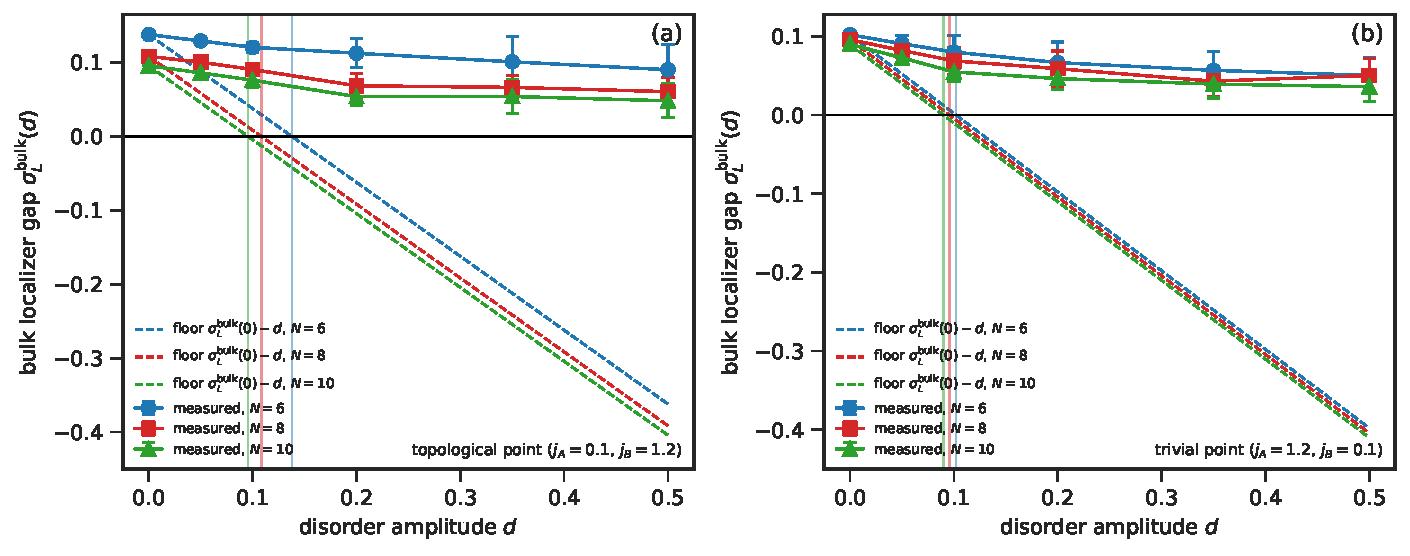
\includegraphics[width=0.9\linewidth]{protection_bound.pdf}
\caption{Disorder resilience of the protection bound at three bulk sizes, for the (a)~topological and (b)~trivial points. Points: measured index-relevant bulk localizer gap (mean over \num{20} disorder realizations, error bars one standard deviation). Dashed lines: linear floor $\sigma_L^{\rm bulk}(0)-d$. Vertical ticks mark $d^\ast$ at each size.}
\label{fig:protection-bound}
\end{figure}

\begin{figure}[t]
\centering
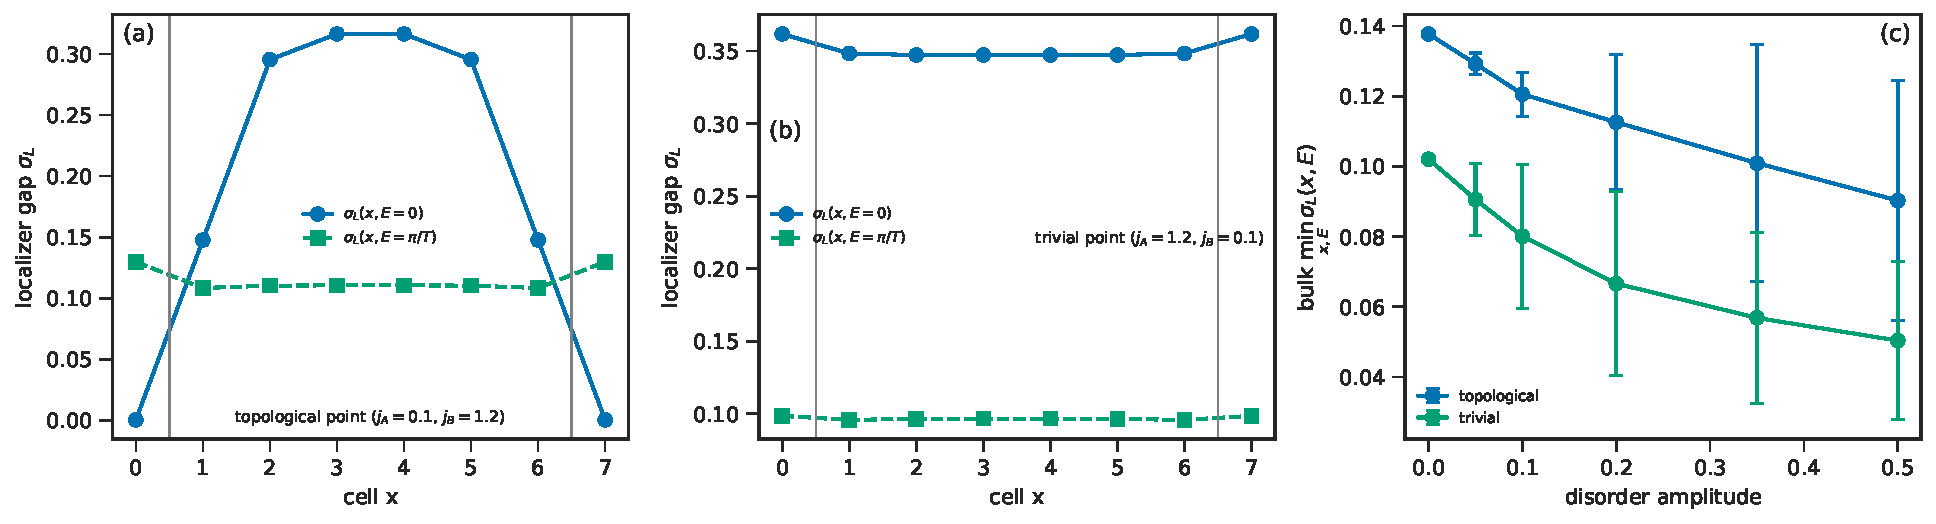
\includegraphics[width=0.9\linewidth]{spectral_localizer.pdf}
\caption{Spectral-localizer certification profiles. (a) Localizer gap versus cell at $N=\num{8}$ for the topological point, and (b) the same for the trivial point, at $E=0$ and $E=\pi/T$. (c) Index-relevant bulk gap versus disorder amplitude ($N=\num{6}$ cells, \num{20} realizations).}
\label{fig:localizer-profiles}
\end{figure}

\subsection{Transfer analysis: when does coherent protection reach the open-system observable?}
\label{sec:localizer-transfer}

The protection bound constrains the single-particle spectrum of the coherent chain. The open-system observable of the main text, the local Wigner negativity $\delta_-(t)$ of the edge site, is a many-body functional of the full dissipative trajectory and is generated at the edge site by the Kerr nonlinearity. The transfer of coherent protection to this functional requires conditions beyond what the localizer gap controls.

\paragraph{Bulk-participation decay bound.}
Let $\ket{e}=\sum_j u_{e,j}\,\ket{j}$ be the single-particle edge mode and let the edge site be $j=\num{0}$. The local negativity satisfies the short-time bound
\begin{equation}\label{eq:participation-bound}
 \delta_-(t)\;\le\;\delta_-(0)\,e^{-\Gamma_{\rm eff}t},
\qquad
 \Gamma_{\rm eff}\;=\;\gamma_0|u_{e,0}|^2+\sum_{j\ne0}\gamma_j|u_{e,j}|^2
 +\gamma_{\rm eb},
\end{equation}
where $\gamma_j$ are the per-site loss rates and $\gamma_{\rm eb}$ is the edge--bulk dephasing rate generated by mode delocalization. Two consequences follow. First, edge-selective loss ($\gamma_0\to0$) removes only the first term; the residual decay $\sum_{j\ne0}\gamma_j|u_{e,j}|^2+\gamma_{\rm eb}$ survives and grows with the bulk participation of the edge mode. Second, as the chain grows the boundary weight $|u_{e,0}|^2$ decreases and the local reduced state is averaged over an increasing number of weakly occupied sites, pushing $W(q,p)$ toward a Gaussian form: a mechanism consistent with the observed sign change of the chiral-minus-trivial contrast between two, three and four cells.

The bound was verified against the chiral primary data (matched-mean final negativity; $\delta_-(0)=\num{0.1962}$ from the identical cat-state edge-site initial condition on the same $\num{31}^2$ Wigner grid). For the edge-low-loss profile at zero disorder, the measured decay rate $\Gamma_{\rm meas}=-\ln[\delta_-(T)/\delta_-(0)]/T$ exceeds the mode-weighted rate $\Gamma_{\rm eff}=\num{0.195}$ at every size, with margins $\num{1.7}$--$\num{3.0}\times$ (\cref{tab:bound-verification}). The residual $\gamma_{\rm eb}=\Gamma_{\rm meas}-\Gamma_{\rm eff}$ grows from \num{0.14} to \num{0.40} as the chain grows, quantitatively consistent with the delocalization mechanism.

\begin{table}[t]
\caption{Verification of the bulk-participation decay bound against the chiral primary data (edge-low-loss profile, zero disorder): the measured decay rate always exceeds the mode-weighted rate.}
\label{tab:bound-verification}
\begin{tabular}{lcccccc}
\hline
Cells & $|u_{e,0}|^2$ & $\Gamma_{\rm eff}$ & $\delta_-(T)$ & $\delta_-(0)$ & $\Gamma_{\rm meas}$ & Ratio \\
\hline
\num{2} ($N_{\rm MC}=\num{500}$) & \num{0.01343} & \num{0.1946} & \num{0.02369} & \num{0.19623} & \num{0.3365} & \num{1.73} \\
\num{3} ($N_{\rm MC}=\num{500}$) & \num{0.01221} & \num{0.1951} & \num{0.00478} & \num{0.19623} & \num{0.5913} & \num{3.03} \\
\num{4} ($N_{\rm MC}=\num{500}$) & \num{0.01220} & \num{0.1951} & \num{0.00478} & \num{0.19623} & \num{0.5913} & \num{3.03} \\
\hline
\end{tabular}
\end{table}

Extending the check to every realization of both loss profiles and all four disorder levels ($\num{24}$ conditions, \num{12000} records), the mean-level ratio $\Gamma_{\rm meas}/\Gamma_{\rm eff}$ is between \num{1.4} and \num{8.4}, and per-realization compliance is \qty{100}{\percent} in \num{20}/\num{24} conditions. The only sub-\qty{100}{\percent} cases are edge-low-loss at disorder $d=\num{1.0}$--\num{1.5} (compliance \qty{77.4}{\percent}--\qty{99.4}{\percent}), where the $\pm$\qty{100}{\percent}--\qty{150}{\percent} rate perturbation drives some realizations' bulk rates far above the mean; there the fixed-mode assumption of the bound is stressed by the disorder, a documented regime boundary rather than a violation of the mean-level statement. At the largest amplitude the same clamping zeroes \emph{every} rate in \qty{14}{\percent}--\qty{16}{\percent} of draws; those realizations evolve without dissipation and are tested against $\delta_-(T)\le\delta_-(0)$.

\begin{table}[t]
\caption{Extended verification of the bound per realization over the full disorder grid ($\num{24}$ conditions, \num{12000} records). The only sub-\qty{100}{\percent} conditions are edge-low-loss at $d=\num{1.0}$--\num{1.5}.}
\label{tab:extended-bound}
\begin{tabular}{lcccc}
\hline
Profile & $d$ & Ratio range & Compliance & \# conditions \\
\hline
edge-low-loss & \num{0.0} & \num{1.73}--\num{2.71} & \qty{100}{\percent} & \num{3} \\
edge-low-loss & \num{0.5} & \num{1.73}--\num{2.80} & \qty{100}{\percent} & \num{3} \\
edge-low-loss & \num{1.0} & \num{1.72}--\num{3.04} & \qty{86.4}{\percent} (\num{2}c); \qty{100}{\percent} (\num{3}c, \num{4}c) & \num{3} \\
edge-low-loss & \num{1.5} & \num{1.38}--\num{2.71} & \qty{77.4}{\percent} (\num{2}c); \qty{99.4}{\percent} (\num{3}c, \num{4}c) & \num{3} \\
uniform & \num{0.0}--\num{1.5} & \num{5.26}--\num{8.41} & \qty{100}{\percent} & \num{12} \\
\hline
\end{tabular}
\end{table}

\paragraph{Closed form of the edge--bulk rate.}
The residual $\gamma_{\rm eb}$ can be computed in closed form from the coherent model. Because the local negativity is a two-photon (cat) coherence of the edge site, its loss exposure is set by the rate-weighted dwell time of the two-photon sector:
\begin{equation}
  \gamma_{\rm eb}\;=\;\kappa\,\Lambda_2^{\rm coh},\qquad
  \Lambda_2^{\rm coh}\;=\;\frac1T\int_0^T\!\!dt
  \!\!\sum_{\substack{i\le j\\(i,j)\neq(0,0)}}\!\!(\gamma_i+\gamma_j)
  \,\bigl|\braket{i,j\,|\,U_2(t)\,|0,0}\bigr|^2,
  \label{eq:gammas-eb-closed}
\end{equation}
where $U_2(t)$ is the two-particle Floquet evolution and $\ket{0,0}$ the two-photon state at the edge site. The prefactor $\kappa=\gamma_{\rm eb}^{\rm meas}/\Lambda_2^{\rm coh}$ is fixed per size by the measured residual. Photon loss on a bare site is a Gaussian channel; its Wigner function evolves by the exact damped-oscillator solution
\begin{equation}\label{eq:fp-loss}
  W_t(\boldsymbol\beta)\;=\;\frac{2}{\pi(1-e^{-\gamma t})}
    \int\!d^2\beta'\,
    \exp\!\Bigl[-\frac{2|\boldsymbol\beta-e^{-\gamma t/2}\boldsymbol\beta'|^2}
      {1-e^{-\gamma t}}\Bigr]\,W_0(\boldsymbol\beta')\,.
\end{equation}
The damping part preserves the integrated negativity $\delta_-$ \emph{exactly}; only the diffusion erodes it. Expanding to first order in $\gamma t$ and verifying against the exact Lindblad flow (\cref{sec:fp-check}) gives $\partial_t W|_{t=0}=\gamma\,[W_0+\tfrac12(\boldsymbol\beta\cdot\nabla)W_0+\tfrac18\Delta W_0]$. With $W_0=0$ on the boundary of the negativity region, the divergence theorem gives
\begin{equation}\label{eq:kappa-single-closed}
  \kappa_{\rm single}\;=\;-\frac1\gamma\,\frac{d\ln\delta_-}{dt}\bigg|_{t=0}
    \;=\;\frac18\,\frac{\int_\Omega\Delta W_0\,d^2\beta}{\delta_-(0)}\,,
\end{equation}
the flux of the Laplacian through the negativity region, normalized by the negativity itself. For the truncated even cat ($N_{\max}=\num{2}$, $\alpha=\num{1}$; $c_0=\num{0.7462}$, $c_2=\num{0.6658}$) this evaluates to $\kappa_{\rm single}=\num{3.411}$, matching the numerically exact short-time slope. In the large-cat limit the same identity returns $2|\alpha|^2$ asymptotically. The single-particle analogue $\Lambda_1$ provides a strict lower bound: $\Lambda_1=\num{0.013}$ (2 cells) and \num{0.052} (3--4 cells), below the measured residuals at every size.

An independent recomputation of \eqref{eq:gammas-eb-closed} with primary parameters (Kerr $k_{\rm Kerr}=\num{0.5}$ on the edge site, edge-low-loss rates, zero disorder) gives $\Lambda_2^{\rm coh}=\num{0.012},\num{0.095},\num{0.095}$ (two, three, four cells; \cref{tab:closedform-kappa}). The structural content that survives independently is: (i)~the strict lower bound $\Lambda_1<\gamma_{\rm eb}^{\rm meas}$ at every size; (ii)~the exact three/four-cell degeneracy, $\Lambda_2^{\rm coh}(3\mathrm{c})=\Lambda_2^{\rm coh}(4\mathrm{c})$, mirroring $\gamma_{\rm eb}^{\rm meas}(3\mathrm{c})\approx\gamma_{\rm eb}^{\rm meas}(4\mathrm{c})$; and (iii)~the boundary jump between two and three cells, present in $\Lambda_2^{\rm coh}$ ($\num{0.012}\to\num{0.095}$) but overpredicted in magnitude (a factor \num{7.9} vs the measured \num{2.79}). The prefactor $\kappa$ is not size-universal ($\num{11.8},\num{4.2},\num{4.2}$ across sizes, a factor \num{2.8} between two and three cells). The closed form is therefore a per-size calibration, not a universal prediction.

\begin{table}[t]
\caption{Independent recomputation of the edge--bulk rate at zero disorder (edge-low-loss profile): $\Lambda_1$ is the strict single-particle lower bound; $\Lambda_2^{\rm coh}$ the rate-weighted two-photon dwell under primary parameters; $\gamma_{\rm eb}^{\rm meas}$ the measured residual; $\kappa$ the per-size prefactor. The exact three/four-cell degeneracy is reproduced under every convention; the prefactor is size-dependent.}
\label{tab:closedform-kappa}
\begin{tabular}{lcccccc}
\hline
Cells & $\Lambda_1$ & $\Lambda_2^{\rm coh}$ & $\Lambda_2^{\rm coh,lin}$ & $\gamma_{\rm eb}^{\rm meas}$ & $\kappa$ & Consistency \\
\hline
\num{2} & \num{0.0128} & \num{0.0120} & \num{0.0256} & \num{0.1419} & \num{11.8} & \num{1.00} \\
\num{3} & \num{0.0523} & \num{0.0950} & \num{0.1046} & \num{0.3962} & \num{4.2} & \num{1.00} \\
\num{4} & \num{0.0523} & \num{0.0950} & \num{0.1046} & \num{0.3962} & \num{4.2} & \num{1.00} \\
\hline
\end{tabular}
\end{table}

\paragraph{Sector dependence of the prefactor.}
Applying the same formula with the same per-size $\kappa_N$ to the trivial sector ($A$ and $B$ interchanged) shows the limits of the linear-loss model. With trivial-sector parameters the site-\num{0} mode is far more edge-concentrated ($|w_0|^2=\num{0.30},\num{0.25},\num{0.17}$ at \num{2},\num{3},\num{4} cells vs.\ \num{0.013} topological), and the measured decay is slower than the transferred prediction by factors \num{3.7}, \num{1.45}, \num{1.51} (effective $\kappa_{\rm eff}=\num{2.86},\num{2.69},\num{2.48}$, decreasing with size). The mode-structure ratio is $\kappa_{\rm topo}/\kappa_{\rm eff}=\num{4.1},\num{1.55},\num{1.68}$: the delocalized topological edge mode converts its small two-photon dwell ($\Lambda_2^{\rm coh}=\num{0.0120}$) into coherence destruction more efficiently than the trivial mode, which spreads the two-photon state over a larger dwell, diluting the coherence over many pair configurations. The closed form reproduces the measured \emph{ordering} of the two-cell rates but not the three- and four-cell sign change: the sign change is a many-body Gaussianization effect that the linear-loss dwell cannot produce.

The two-to-three-cell jump is consistent with a boundary effect of the mode delocalization: the inter-cell Floquet step transfers the edge-site excitation to site $j=\num{3}$ with a period-averaged dwell $\langle P_3\rangle_T=\num{0.198}$, and the single-particle dwell profile is identical at all chain lengths. In the two-cell chain site \num{3} is the opposite edge ($\gamma_3=\qty{1e-4}{}$), so the visiting population is shielded; from three cells on it is a bulk site ($\gamma_3=\num{0.2}$) and the same dwell is exposed to the bulk loss rate. The rate-weighted integrals inherit exactly this boundary dependence.

This lemma is the negative side of the mixed-state-SPT lesson discussed in the main text: the localizer gap pins the coherent sector, but the negativity survives only to the extent that its generating mode stays localized at the measured site. The collective null result is consistent with \cref{eq:participation-bound}: the collective edge mode is the same sector vector $c$ with bulk participation $1-|c_0|^2=\num{0.987}$, so its marginal is already Gaussian at $t=\num{0}$ ($\delta_-(0)=\num{0}$) and the bound is satisfied trivially in every record at both Fock truncations and both sizes. The closed form over-determines this null result: the collective two-photon state $\ket{c,c}$ is itself an (almost) stationary eigenmode of the two-particle Floquet operator, so its dwell is static and fully bulk-exposed ($\Lambda_2^{\rm coh}=\num{0.3925}$ for two cells and \num{0.3952} for three--four cells; $\Lambda_1=\num{0.195}$). No $\gamma_{\rm eb}$ or total decay rate is inferred from the collective null; its $\Gamma_{\rm eff}^{\rm tot}\approx\num{1.32}$ is the largest in the model. The local mode retains a positive weight $|u_{e,0}|^2=\num{0.013}>0$ and is the only marginal able to sustain the observed positive contrast under edge-selective loss.

\begin{table}[t]
\caption{Collective-mode Wigner null and dwell diagnostic (edge-low-loss, zero disorder). The collective marginal is Gaussian at $t=\num{0}$ and remains zero in all tested records. The reported dwell values are structural diagnostics; no universal prefactor or inferred $\gamma_{\rm eb}$ is claimed.}
\label{tab:collective-null}
\begin{tabularx}{\linewidth}{lcX}
\hline
Quantity & Collective edge mode & Local site \num{0} \\
\hline
Edge weight $|c_0|^2=|u_{e,0}|^2$ & \num{0.01343} & \num{0.01343} \\
Bulk participation $1-|c_0|^2$ & \num{0.9866} & \num{0.9866} \\
$\delta_-(0)$ (identical cat) & \num{0.000000} & \num{0.1962} \\
$\Lambda_1$ & \num{0.195} & \num{0.013} (\num{2}c) / \num{0.052} (\num{3}--\num{4}c) \\
$\Lambda_2^{\rm coh}$ & \num{0.3925} (\num{2}c) / \num{0.3952} (\num{3}--\num{4}c) & \num{0.012} (\num{2}c) / \num{0.095} (\num{3}--\num{4}c) \\
$\Gamma_{\rm eff}$ diagnostic & not inferred & \num{0.337} (\num{2}c) / \num{0.591} (\num{3}--\num{4}c) \\
$\delta_-(T)$ (data) & \num{0.000000} in \num{320}/\num{320} & \num{0.0237} (\num{2}c) / \num{0.0048} (\num{3}c) \\
\hline
\end{tabularx}
\end{table}

\section{Physical parameter mapping and hardware bounds}
\label{sec:hardware}

The main text uses normalized model coordinates ($T=2\pi$, all rates in units of $\omega_d=2\pi/T$). This section gives an \emph{illustrative} mapping to concrete hardware so the dimensionless content can be compared with real platforms. It is not a calibration. Any normalized rate $\Gamma$ becomes $\Gamma\,\omega_d$. For a superconducting platform at $\omega_d/2\pi=\qty{100}{MHz}$ ($T=\qty{10}{ns}$): $J_B\simeq\qty{754}{MHz}$, $\chi\simeq\qty{314}{MHz}$, $\gamma_{\rm bulk}\simeq\qty{126}{MHz}$, $\gamma_{\rm edge}\simeq\qty{63}{kHz}$, $J_A\simeq\qty{63}{MHz}$. For an optomechanical platform at $\omega_d/2\pi=\qty{10}{MHz}$: $J_B\simeq\qty{75}{MHz}$, $\chi\simeq\qty{31}{MHz}$, $\gamma_{\rm bulk}\simeq\qty{13}{MHz}$, $\gamma_{\rm edge}\simeq\qty{6.3}{kHz}$, $J_A\simeq\qty{6.3}{MHz}$. The ratios $\chi/J_B=\num{0.42}$, $\gamma_{\rm bulk}/\chi=\num{0.4}$, and $\gamma_{\rm edge}/\gamma_{\rm bulk}=\num{5e-4}$ are preserved in both rows. Hopping of tens to hundreds of megahertz, Kerr of a few hundred megahertz, and quality factors of order $10^4$ are within reach of tunable-coupler transmon arrays~\cite{Blais2021Circuit}; on the optomechanical side~\cite{Xuereb2014}, phonon hopping in the megahertz range with kilohertz--megahertz mechanical loss is standard.

The measurement chain uses established primitives: parity-based direct Wigner reconstruction~\cite{Lutterbach1997}, macroscopic cavity cat states in circuit QED~\cite{Vlastakis2013}, and dissipatively stabilized quantum manifolds~\cite{Touzard2018}, with a standard homodyne chain on the optomechanical side~\cite{Aspelmeyer2014}. The grid-free witness of \cref{sec:witness} requires only displaced photon-number statistics, so detecting the two-cell signal needs a finite set of displaced measurements rather than full tomography. Site selectivity follows from frequency-resolved cavity modes addressed by a shared ancilla~\cite{Blais2021Circuit}. The engineered bulk loss corresponds to dissipative stabilization of a dynamical manifold~\cite{Touzard2018}.

\Cref{tab:testable} collects the concrete testable predictions. The near-term target is the two-cell witness asymmetry (\qty{82.4}{\percent} versus \qty{10.8}{\percent} single-shot certification rates, a few hundred repetitions with no tomography). The full sign pattern is a tomography-level prediction at sub-$\num{1e-3}$ resolution. Every entry is conditional on stroboscopic readout at $t=T$ and on the structured loss profile ($\gamma_{\rm edge}/\gamma_{\rm bulk}=\num{5e-4}$); micromotion predicts sign changes within the period, and the loss-ratio scan predicts the signal to vanish by ratio \num{0.5}.

\begin{table}[!htbp]
\renewcommand{\arraystretch}{1.3}
\caption{Testable predictions of the present study. All values requote primary results; none is a new fit.}
\label{tab:testable}
\begin{tabularx}{\linewidth}{lXX}
\hline
Prediction & Measurement & Expected outcome \\
\hline
Two-cell witness asymmetry & Displaced photon counting & \qty{82.4}{\percent} vs \qty{10.8}{\percent} (disjoint Wilson intervals) \\
Contrast sign pattern, 2--5 cells & Wigner tomography at $t=T$ & $+\num{0.017}$ at two cells; $-\num{0.002}$ at three to five cells \\
Kerr-free sign pattern & Same, nonlinearity off & Same signs; two-cell contrast $\num{2.1}\times$ smaller \\
Uniform-loss null & Same, uniform profile & Contrast at \num{1e-6} level at $t=T$ \\
Stroboscopic conditioning & Readout at $t\ne T$ & Sign changes within every period \\
Loss-ratio dependence & Vary edge-to-bulk ratio & Signal gone by ratio \num{0.5} \\
Five-cell sign & Ten-mode tomography & Negative, inside pre-specified interval \\
\hline
\end{tabularx}
\end{table}

The reported contrasts are invariant under a uniform rescaling of $\omega_d$; the physical time over which the sign flip occurs is $T\sim\qtyrange{10}{100}{ns}$, well below typical coherence times. The normalized study does not include measurement back-action or drive-induced heating; the mapping bounds idealized-device predictions, not hardware.

\subsection{Step-by-step measurement protocol}
\label{sec:measurement-protocol}

Each step states its setting, check, and acceptance criterion. No step requires model fitting.

\begin{enumerate}
\item \emph{Prerequisites.} An array of \num{4}--\num{10} bosonic modes with site-resolved readout, tunable nearest-neighbour couplings, a Kerr nonlinearity on the edge site, and engineered loss with edge-to-bulk contrast at least two orders of magnitude. Multimode cats have been stabilized by normal-mode dissipation engineering~\cite{Zapletal2022multimode} and cat manifolds by nonlinear reservoir engineering~\cite{Rojkov2026catmanifolds}.
\item \emph{Coherent calibration.} Working points $(J_A,J_B)=(\num{0.1},\num{1.2})$ (chiral) and $(\num{1.2},\num{0.1})$ (control). Accept when spectroscopy reproduces the minimum zero and $\pi$ quasienergy gaps \num{2.1991} and \num{0.3142} and edge modes appear at the chiral point only.
\item \emph{Loss engineering.} $\gamma_{\rm bulk}=\num{0.2}$, $\gamma_{\rm edge}=\num{1e-4}$ (drive units). Accept when ringdown reproduces both rates with ratio below \num{1e-2}.
\item \emph{State preparation.} Even cat $\alpha=\num{1}$ on site~\num{0}. Accept when pre-drive local Wigner negativity reads $\delta_-(\num{0})=\num{0.1962}$.
\item \emph{Single-period drive.} Read out at $t=T$ locked to the drive phase. This lock is mandatory: micromotion predicts sign changes within the period.
\item \emph{Witness measurement (near-term target).} Displaced photon counting for the $F_1$ witness against $\omega_1=\num{0.5}$. Separating \qty{82.4}{\percent} vs \qty{10.8}{\percent} needs \num{7} shots per sector at \qty{80}{\percent} power and \num{10} at \qty{95}{\percent}; \num{300} shots give Wilson half-widths below \num{0.05}. Accept when the two intervals are disjoint and ordered.
\item \emph{Tomography (full pattern).} Edge-site Wigner function on $\num{31}^2$ grid (\num{961} settings per function) for both sectors. Accept $+\num{0.0167}\pm\num{0.0011}$ (two cells), $-\num{0.0021}\pm\num{0.0011}$ (three and four cells), $-\num{0.0022}\pm\num{0.0007}$ (five cells); $\approx\num{0}$ under uniform profile.
\item \emph{Disorder and sweep repetition.} Repeat steps 4--7 over disorder amplitudes \num{0}--\num{1.5} (\num{500} matched units per setting at two and three cells) and along $J_A+J_B=\num{1.3}$. Accept when the contrast stays continuous through all three closings with a zero window straddling the $\nu_0$ transition.
\item \emph{Falsification.} The boundary claim fails if the contrast tracks the invariant across the transition, or if a nonzero uniform-loss contrast appears at $t=T$, or if the five-cell sign falls outside the pre-specified interval.
\end{enumerate}

\section{Short-time Lindblad expansion in the truncated space}
\label{sec:fp-check}

The short-time expansion underlying \eqref{eq:kappa-single-closed} is verified in closed form against the exact Lindblad flow. In the truncated $N_{\max}=\num{2}$ space the even cat is $\ket{\psi}=c_0\ket{0}+c_2\ket{2}$ with $c_0=\num{0.7462}$, $c_2=\num{0.6658}$. The ideal untruncated even cat has Fock weights \qty{64.8}{\percent} ($n=\num{0}$), \qty{32.4}{\percent} ($n=\num{2}$), \qty{2.79}{\percent} ($n\ge\num{4}$), so the primary construction excludes the $n\ge\num{4}$ tail by design. The amplitude-damping channel $\dot\rho=\gamma(a\rho a^\dagger-\tfrac12\{a^\dagger a,\rho\})$ closes on the diagonal and coherence elements
\begin{equation}\label{eq:lindblad-trunc}
  \rho_{22}(t)=c_2^2e^{-2\gamma t},\qquad
  \rho_{11}(t)=2c_2^2\gamma t\,e^{-\gamma t},\qquad
  \rho_{02}(t)=e^{-\gamma t}\bigl[c_0c_2+c_2^2\gamma^2t^2\bigr],
\end{equation}
with $\rho_{00}=1-\rho_{11}-\rho_{22}$. Inserting into the Wigner function $W_t=(2/\pi)e^{-2r}[\rho_{00}+\rho_{11}(4r-1)+\rho_{22}(1-8r+8r^2)+4\sqrt2\,\rho_{02}(x^2-y^2)]$ and expanding to first order in $\gamma t$ gives, identically in $r$ and $x^2-y^2$, $\partial_t W|_{t=0}=\gamma[W_0+\tfrac12(\boldsymbol\beta\cdot\nabla)W_0+\tfrac18\Delta W_0]$, the same expansion obtained from \eqref{eq:fp-loss}. The two independent derivations (Gaussian-channel solution and exact Lindblad flow) therefore agree to all orders needed for \eqref{eq:kappa-single-closed}.

\section{Scope and limitations}
\label{sec:scope-limitations}

\begin{table}[!htbp]
\renewcommand{\arraystretch}{1.35}
\caption{Scope of the conclusions for the results presented in the main text and Supplemental Material.}
\label{tab:scope-limitations}
\begin{tabularx}{\linewidth}{lX}
\textbf{Quantity} & \textbf{Interpretation} \\
\hline
Chiral bulk invariant & Reproduced by two independent implementations (frame winding and spectral localizer). \\\hline
Finite-chain edge state & Model-level observable. \\\hline
Paired trajectories and finite-value analysis & Supported for the stated comparison. \\\hline
Size-robust local Wigner protection & Not supported by the data. \\\hline
Passive edge-mode reference & Not established. \\\hline
Cutoff convergence of reference & Not established. \\\hline
Local-negativity cutoff dependence & Reported descriptively; not converged. \\\hline
Wigner-grid discretization & Within $\pm\qty{3}{\percent}$ of the finest grid. \\\hline
Trajectory-count sensitivity & $\approx\qty{4}{\percent}$ on a fixed realization; contrast ladder in \cref{sec:trajcount}. \\\hline
Collective-mode Wigner negativity & Not established; measured as null for both preparations (\cref{sec:collective-wigner}). \\\hline
Multi-period behavior & No sign inversion up to eight periods; two-cell revival at four periods (\cref{sec:multiperiod}). \\\hline
Edge-to-bulk loss-ratio dependence & Positive four-mode contrast requires the sharp engineered profile; lost for ratio \num{5e-1}. \\\hline
Eight-mode statistical power & Resolves $|\Delta|\gtrsim\num{0.00077}$ at $N_{\rm MC}=\num{2000}$; observed mean $\approx\num{2.6}\times$ the resolution. \\\hline
Correspondence with the bulk invariant & Not established: contrast is continuous at all three gap closings and identically zero on a window straddling the $\nu_0$ change. \\\hline
Chiral-symmetry-compatible dissipation & Not protective: strong-symmetry sublattice loss gives a small resolved negative contrast, unchanged under budget matching. \\\hline
Phase of the drive at measurement & Order-of-magnitude swing and sign change within one period in every tested condition. \\\hline
Five-cell size & Predicted out of sample: \num{4} of \num{4} conditions inside the pre-specified interval; negative branch saturates near \num{0.0021}. \\\hline
Grid-free negativity certification & Displaced Fock-state witnesses detect the two-cell signal in \qty{82.4}{\percent} versus \qty{10.8}{\percent} of draws. \\\hline
Long-time sign persistence & No reversal over \num{64} periods; both branches decay to the numerical floor. \\\hline
Physical calibration and optimality & Not computed. \\
\end{tabularx}
\end{table}

The limits in \cref{tab:scope-limitations} confine the conclusions to the coherent-sector calculations, the finite-time open-system comparison, and the specified deterministic calculations.

\bibliographystyle{apsrev4-2}
\bibliography{references}

\end{document}
